\documentclass{AeroStructure-ERJohnson}
\input crosslink.tex

%\usepackage{showframe}
\def\ShowFrameLinethickness{0.125pt}

\allowdisplaybreaks

\def\harp#1{\smash{\mathord{\buildrel{\lower3pt\hbox{$\scriptscriptstyle\rightharpoonup$}}\over{#1}}}}
%\def\tfrown#1{\smash{\stackrel{\raisebox{-2pt}{$\frown$}}{#1}}}
\def\tfrown#1{\overset{\smash{\lower3pt\hbox{$\frown$}}}{#1}}


%\myexternaldocument{App_4P}
\myexternaldocument{Ch01_4P}
\myexternaldocument{Ch02_4P}
\myexternaldocument{Ch03_4P}
\myexternaldocument{Ch04_4P}
\myexternaldocument{Ch05_4P}
\myexternaldocument{Ch06_4P}
\myexternaldocument{Ch07_4P}
\myexternaldocument{Ch08_4P}
\myexternaldocument{Ch09_4P}
\myexternaldocument{Ch10_4P}
\myexternaldocument{Ch11_4P}
\myexternaldocument{Ch12_4P}
\myexternaldocument{Ch13_4P}
\myexternaldocument{Ch14_4P}
\myexternaldocument{Ch15_4P}
\myexternaldocument{Ch16_4P}
\myexternaldocument{Ch17_4P}
\myexternaldocument{Ch18_4P}



\begin{document}
\mainmatter

%\hbox{~}\clearpage
%\setcounter{page}{533}


\appendix

\chapter{Linear elasticity of solid bodies} \label{appendix}

Solid mechanics is a branch of continuum mechanics that studies the behavior of solid materials under the action of forces, temperature changes, or other external agents. Elasticity is a branch of solid mechanics that refers to the ability of the body to return to its original size and shape after the forces causing deformation are removed. In this appendix the basic equations of the three-dimensional elasticity theory are developed at a material point in the body. A material point, or particle, is identified by its position in a rectangular Cartesian coordinate system $(x_{1},x_{2},x_{3})$. The fundamental equations of elasticity consist of the geometry of deformation in article~\ref{secA.1}, the stresses and equilibrium in article~\ref{secA.2}, and the stress-deformation relations in article~\ref{secA.3}. The focus is on the classical linear elasticity theory in which the strains are small with respect to unity and the material is linear elastic. The basic equations are summarized in article~\ref{secA.4} along with a description of the boundary value problems of elasticity.


\section{Geometry of deformation}\label{secA.1}

A continuous three-dimensional body occupies a closed region denoted by $B_{0}$ in the reference state. Let every point of $B_{0}$ be defined in a fixed rectangular Cartesian system of axes $x_{1}$, $x_{2}$, and $x_{3}$. Let $B$ denote the closed region of the body after it undergoes a deformation. The position vector of the point $P_{0}$ in region $B_{0}$ with respect to the origin is
\begin{equation}
\harp{r}=x_{1}\hat{i}_{1}+x_{2}\hat{i}_{2}+x_{3}\hat{i}_{3}, \label{eqA.1}
\end{equation}
\noindent where the unit vectors along the fixed axes are $\hat{i}_{1}$, $\hat{i}_{2}$, and $\hat{i}_{3}$. The particle at $P_{0}{:}(x_{1}, x_{2}, x_{3})$ passes to point $P{:}(y_{1}, y_{2}, y_{3})$ in region $B$, where coordinates $(y_1, y_{2}, y_{3})$ are defined in the same fixed coordinate system. See figure~\ref{figA.1}. The position vector of point $P$ referred to the same origin is

\processfigure{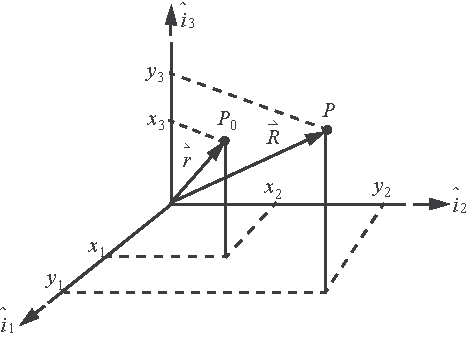
\includegraphics{Figure_A-1.pdf}
}{\caption{A particle at point $P_{\textbf{0}}{:}(x_{\textbf{1}}, x_{\textbf{2}}, x_{\textbf{3}})$ in the reference configuration of the body and its position $P_{\textbf{0}}{:}(y_{\textbf{1}},y_{\textbf{2}},y_{\textbf{3}})$ in the body after deformation.\label{figA.1}}}

\vspace*{-1pc}

\begin{equation}
\harp{R}=y_{1} \hat{i}_{1}+y_{2} \hat{i}_{2}+y_{3} \hat{i}_{3}. \label{eqA.2}
\end{equation}
The deformation of the body is defined by the equations
\begin{equation}
y_{1}=y_{1}(x_{1}, {x}_{2}, x_{3}) \quad y_{1}=y_{2}(x_{1}, {x}_{2}, x_{3}) \quad y_{3}=y_{3}(x_{1}, {x}_{2}, x_{3}), \label{eqA.3}
\end{equation}
where $ x_{1}$, $x_{2}$, and $x_{3}$ are restricted to $B_{0}$ and $y_{1}$, $y_{2}$, and $y_{3}$ are restricted to $B$.  In eq. (\ref{eqA.3}) the $y_{i}$, $i=1,2,3$, on the right-hand side denotes a function of three variables $x_{1}$, $x_{2}$, and $x_{3}$, and $y_{i}$ on the left-hand side denotes the value of the function. Equation (\ref{eqA.3}) defines the final location of the particle in $B$ that is located at point $P_{0}$ in $B_{0}$. To prohibit the possibility that a particle at point $P$ in region $B$ maps to more than one point in region $B_{0}$, or vice versa, it is required that there is a one-to-one correspondence between points in regions $B_{0}$ and $B$. It follows that in region $B$ eq. (\ref{eqA.3}) has single-valued solutions:
\begin{align}\label{eqA.4}
x_{1}=x_{1}(y_{1}, y_{2}, y_{3}) \quad x_{2}=x_{2}(y_{1}, y_{2}, y_{3}) \quad x_{3}=x_{3}(y_{1}, y_{2}, y_{3}).
\end{align}
The functions defined in eqs. (\ref{eqA.3}) and (\ref{eqA.4}) are assumed to be continuous and differentiable in their respective variables. Continuity insures no fracture of the body results in the deformation. If we choose eq. (\ref{eqA.3}) to describe the deformation of the body then $ x_{1}$, $x_{2}$, and  $x_{3}$ are the independent variables, and the formulation is called the Lagrangian or the referential or material description. In the Lagrangian formulation we follow the particle originally at point $P_{0}{:}(x_{1}, x_{2}, x_{3})$ as the deformation proceeds. If we choose eq. (\ref{eqA.4}) to describe the deformation of the body, then $ y_{1}$, $y_{2}$, and $y_{3}$ are the independent variables, and the formulation is called the Eulerian or spatial description. In the Eulerian formulation the same fixed spatial position $y_{1}$, $y_{2}$, $y_{3}$ is occupied by different particles as the deformation proceeds. The Lagrangian description of the deformation is selected for the developments that follow in this appendix. The position vector of point $P$ relative to point $P_{0}$ is denoted by $\harp{u}$ and is called the displacement vector. Thus,
\begin{align}\label{eqA.5}
\harp{u}=\harp{R}-\harp{r}=\left(y_{1}-x_{1}\right) \hat{i}_{1}+\left(y_{2}-x_{2}\right) \hat{i}_{2}+\left(y_{3}-x_{3}\right) \hat{i}_{3}.
\end{align}
Components of the displacement vector are
\begin{align}\label{eqA.6}
\begin{split}
u_{1}(x_{1}, x_{2}, x_{3})=y_{1}(x_{1}, x_{2}, x_{3})-x_{1} \\
u_{2}(x_{1}, x_{2}, x_{3})=y_{2}(x_{1}, x_{2}, x_{3})-x_{2} \\
u_{3}(x_{1}, x_{2}, x_{3})=y_{3}(x_{1}, x_{2}, x_{3})-x_{3}
\end{split}.
\end{align}
\begin{figure}
\centering{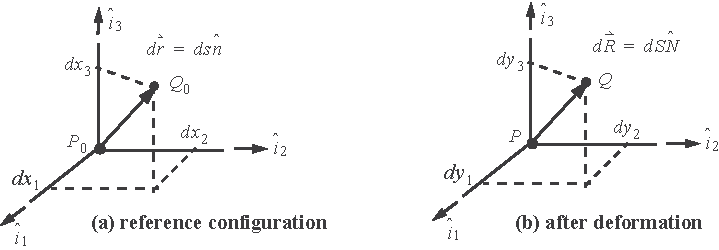
\includegraphics{Figure_A-2.pdf}}
\caption{(a) Line element $\protect\tfrown{P_{\textbf{0}}Q_{\textbf{0}}}$ passes to (b) line element $\protect\tfrown{PQ}$.\label{figA.2}}
\end{figure}
\indent Deformation is quantified by the change in distance between any two points in a body. Consider two infinitesimally close points $P_{0}$ and $Q_{0}$ in region $B_{0}$ that pass to points $P$ and $Q$, respectively, in region $B$. The differential line element $\tfrown{P_{0} Q_{0}}$ in region $B_{0}$ shown in figure~\ref{figA.2}(a) passes to the differential line element $\tfrown{PQ}$ in region $B$ shown in figure~\ref{figA.2}(b). The differential position vector of line element $\tfrown{P_{0} Q_{0}}$ is $d \harp{r}=d x_{1} \hat{i}_{1}+d x_{2} \hat{i}_{2}+d x_{3} \hat{i}_{3}$. The square of the length of $d \harp{r}$ is given by $d s^{2}=d \harp{r} \bullet d \harp{r}=(d x_{1})^{2}+(d x_{2})^{2}+(d x_{3})^{2}$. The unit vector of point $Q_{0}$ with respect to point $P_{0}$ is given by
\begin{align}\label{eqA.7}
\hat{n}=\frac{d \harp{r}}{d s}=\frac{d x_{1}}{d s} \hat{i}_{1}+\frac{d x_{2}}{d s} \hat{i}_{2}+\frac{d x_{3}}{d s} \hat{i}_{3}.
\end{align}
Write unit vector in eq. (\ref{eqA.7}) as
\begin{align}\label{eqA.8}
\hat{n}=n_{1} \hat{i}_{1}+n_{2} \hat{i}_{2}+n_{3} \hat{i}_{3},
\end{align}
where $n_{i}=\frac{d x_{i}}{d s}$, $i=1,2,3$. The differential position vector of $\tfrown{PQ}$ is $d \harp{R}=d y_{1} \hat{i}_{1}+d y_{2} \hat{i}_{2}+d y_{3} \hat{i}_{3}$, and the square of its length is $d S^{2}=d \harp{R} \bullet d \harp{R}=(d y_{1})^{2}+(d y_{2})^{2}+(d y_{3})^{2}$. Write the differential vector as $d\harp{R}=d S \hat{N}$ where the unit vector of point $Q$ with respect to point $P$ is
\begin{align}\label{eqA.9}
\hat{N}=\frac{d y_{1}}{d S} \hat{i}_{1}+\frac{d y_{2}}{d S} \hat{i}_{2}+\frac{d y_{3}}{d S} \hat{i}_{3}=N_{1} \hat{i}_{1}+N_{2} \hat{i}_{2}+N_{3} \hat{i}_{3}
\end{align}
The total differentials $(d y_{1}, d y_{2}, d y_{3})$ of the functions $y_{1}(x_{1}, x_{2}, x_{3})$, $y_{2}(x_{1}, x_{2}, x_{3})$, and $y_{3}(x_{1}, x_{2}, x_{3})$ are written in terms of the total differentials $(d x_{1}, d x_{2}, d x_{3})$ by
\begin{align}\label{eqA.10}
\left[\begin{array}{@{}l@{}} d y_{1} \\ d y_{2} \\ d y_{3} \end{array}\right]=\left[\begin{array}{@{}lll@{}} \displaystyle\frac{\partial y_{1}}{\partial x_{1}} & \displaystyle\frac{\partial y_{1}}{\partial x_{2}} & \displaystyle\frac{\partial y_{1}}{\partial x_{3}} \\[11pt] \displaystyle\frac{\partial y_{2}}{\partial x_{1}} & \displaystyle\frac{\partial y_{2}}{\partial x_{2}} & \displaystyle\frac{\partial y_{2}}{\partial x_{3}} \\[11pt] \displaystyle\frac{\partial y_{3}}{\partial x_{1}} & \displaystyle\frac{\partial y_{3}}{\partial x_{2}} & \displaystyle\frac{\partial y_{3}}{\partial x_{3}} \end{array}\right]\left[\begin{array}{@{}c@{}} d x_{1} \\ d x_{2} \\ d x_{3} \end{array}\right].
\end{align}
The determinate of the 3X3 matrix in eq. (\ref{eqA.3}) is
\begin{align}\label{eqA.11}
J=\operatorname{\it det}\left[\begin{array}{@{}lll@{}} \displaystyle\frac{\partial y_{1}}{\partial x_{1}} & \displaystyle\frac{\partial y_{1}}{\partial x_{2}} & \displaystyle\frac{\partial y_{1}}{\partial x_{3}} \\[11pt] \displaystyle\frac{\partial y_{2}}{\partial x_{1}} & \displaystyle\frac{\partial y_{2}}{\partial x_{2}} & \displaystyle\frac{\partial y_{2}}{\partial x_{3}} \\[11pt] \displaystyle\frac{\partial y_{3}}{\partial x_{1}} & \displaystyle\frac{\partial y_{3}}{\partial x_{2}} & \displaystyle\frac{\partial y_{3}}{\partial x_{3}} \end{array}\right],
\end{align}
where $J$ is called the Jacobian. Equation (\ref{eqA.3}) possesses a continuous single-valued solution satisfying the inverse (\ref{eqA.4}) if and only if the Jacobian is positive for all points in region $B_{0}$ (Batra, 2006). The strain of line element $\tfrown{PQ}$ is defined by
\begin{align}\label{eqA.12}
\varepsilon_{L}=\frac{1}{2}\left[\frac{d S^{2}-d s^{2}}{d s^{2}}\right]=\frac{1}{2}\left[\left(\frac{d S}{d s}\right)^{2}-1\right].
\end{align}
Use the chain rule to write the square of the length of line element $\tfrown{PQ}$ with respect to the square of the length of   line element $\tfrown{P_{0} Q_{0}}$ as
\begin{align}\label{eqA.13}
d S^{2}=\left[\left(\frac{d y_{1}}{d s}\right)^{2}+\left(\frac{d y_{2}}{d s}\right)^{2}+\left(\frac{d y_{2}}{d s}\right)^{2}\right] d s^{2}.
\end{align}
From eq. (\ref{eqA.10}) use the chain rule again to write the differential $ d y_{1} $ as follows:
\begin{align}\label{eqA.14}
d y_{1}=\frac{\partial y_{1}}{\partial x_{1}} d x_{1}+\frac{\partial y_{1}}{\partial x_{2}} d x_{2}+\frac{\partial y_{1}}{\partial x_{3}} d x_{3}=\left[\frac{\partial y_{1}}{\partial x_{1}} \frac{d x_{1}}{d s}+\frac{\partial y_{1}}{\partial x_{2}} \frac{d x_{2}}{d s}+\frac{\partial y_{1}}{\partial x_{3}} \frac{d x_{3}}{d s}\right] d s.
\end{align}
\looseness-1Substitute $d x_{i} / d s=n_{i}$ from eq. (\ref{eqA.8}), and substitute $u_{1}+x_{1}$ for coordinate $y_{1}$ from eq. (\ref{eqA.6}), into eq. (\ref{eqA.14})~to~get
\begin{align}\label{eqA.15}
\frac{d y_{1}}{d s}=\left[\left(1+\frac{\partial u_{1}}{\partial x_{1}}\right) n_{1}+\frac{\partial u_{1}}{\partial x_{2}} n_{2}+\frac{\partial u_{1}}{\partial x_{3}} n_{3}\right].
\end{align}
Starting with differentials $d y_{2}$ and $d y_{3}$ from eq. (\ref{eqA.10}), we perform similar manipulations leading to eq. (\ref{eqA.15}) to find
\begin{align}\label{eqA.16}
\frac{d y_{2}}{d s}=\left[\frac{\partial u_{2}}{\partial x_{1}} n_{1}+\left(1+\frac{\partial u_{2}}{\partial x_{2}}\right) n_{2}+\frac{\partial u_{2}}{\partial x_{3}} n_{3}\right] \quad \frac{d y_{3}}{d s}=\left[\frac{\partial u_{3}}{\partial x_{1}} n_{1}+\frac{\partial u_{3}}{\partial x_{2}} n_{2}+\left(1+\frac{\partial u_{3}}{d x_{3}}\right) n_{3}\right].
\end{align}
Substitute eq. (\ref{eqA.13}) into eq. (\ref{eqA.12}) to write the equivalent expression for the strain in eq. (\ref{eqA.12}) as
\begin{align}\label{eqA.17}
\varepsilon_{L}=\frac{1}{2}\left[\left(\frac{d y_{1}}{d s}\right)^{2}+\left(\frac{d y_{2}}{d s}\right)^{2}+\left(\frac{d y_{2}}{d s}\right)^{2}-\left(n_{1}^{2}+n_{2}^{2}+n_{3}^{2}\right)\right],
\end{align}
where the number one that appears in eq. (\ref{eqA.12}) is replaced by $n_{1}^{2}+n_{2}^{2}+n_{3}^{2}$. Substitute the results from eqs. (\ref{eqA.15}) and (\ref{eqA.16}) into eq. (\ref{eqA.17}) and write the result as
\begin{align}\label{eqA.18}
\varepsilon_{L}=\varepsilon_{11} n_{1}^{2}+\varepsilon_{12} n_{1} n_{2}+\varepsilon_{13} n_{1} n_{3}+\varepsilon_{21} n_{2} n_{1}+\varepsilon_{22} n_{2}^{2}+\varepsilon_{23} n_{2} n_{3}+\varepsilon_{31} n_{3} n_{1}+\varepsilon_{32} n_{3} n_{2}+\varepsilon_{33} n_{3}^{2}.
\end{align}
The expression (\ref{eqA.18}) for the strain can be written in the matrix form
\begin{align}\label{eqA.19}
\varepsilon_{L}=\left[\begin{array}{@{}lll@{}}n_{1} & n_{2} & n_{3}\end{array}\right]\left[\begin{array}{@{}lll@{}}\varepsilon_{11} & \varepsilon_{12} & \varepsilon_{13} \\\varepsilon_{21} & \varepsilon_{22} & \varepsilon_{23} \\\varepsilon_{31} & \varepsilon_{32} & \varepsilon_{33}\end{array}\right]\left[\begin{array}{@{}c@{}}n_{1} \\n_{2} \\n_{3}\end{array}\right].
\end{align}
The coefficients in the expression for the strain  are as follows:
\begin{gather}\label{eqA.20}
\varepsilon_{11}=\frac{\partial u_{1}}{\partial x_{1}}+\frac{1}{2}\left[\left(\frac{\partial u_{1}}{\partial x_{1}}\right)^{2}+\left(\frac{\partial u_{2}}{\partial x_{1}}\right)^{2}+\left(\frac{\partial u_{3}}{\partial x_{1}}\right)^{2}\right]\\
\label{eqA.21}\varepsilon_{22}=\frac{\partial u_{2}}{\partial x_{2}}+\frac{1}{2}\left[\left(\frac{\partial u_{1}}{\partial x_{2}}\right)^{2}+\left(\frac{\partial u_{2}}{\partial x_{2}}\right)^{2}+\left(\frac{\partial u_{3}}{\partial x_{2}}\right)^{2}\right]\\
\label{eqA.22}	\varepsilon_{33}=\frac{\partial u_{3}}{\partial x_{3}}+\frac{1}{2}\left[\left(\frac{\partial u_{1}}{\partial x_{3}}\right)^{2}+\left(\frac{\partial u_{2}}{\partial x_{3}}\right)^{2}+\left(\frac{\partial u_{3}}{\partial x_{3}}\right)^{2}\right]\\
\label{eqA.23}	\varepsilon_{12}=\varepsilon_{21}=\frac{1}{2}\left[\frac{\partial u_{1}}{\partial x_{2}}+\frac{\partial u_{2}}{\partial x_{1}}+\frac{\partial u_{1}}{\partial x_{1}} \frac{\partial u_{1}}{\partial x_{2}}+\frac{\partial u_{2}}{\partial x_{1}} \frac{\partial u_{2}}{\partial x_{2}}+\frac{\partial u_{3}}{\partial x_{1}} \frac{\partial u_{3}}{\partial x_{2}}\right]\\
\label{eqA.24}	\varepsilon_{13}=\varepsilon_{31}=\frac{1}{2}\left[\frac{\partial u_{1}}{\partial x_{3}}+\frac{\partial u_{3}}{\partial x_{1}}+\frac{\partial u_{1}}{\partial x_{1}} \frac{\partial u_{1}}{\partial x_{3}}+\frac{\partial u_{2}}{\partial x_{1}} \frac{\partial u_{2}}{\partial x_{3}}+\frac{\partial u_{3}}{\partial x_{1}} \frac{\partial u_{3}}{\partial x_{3}}\right]\\
\label{eqA.25}	\varepsilon_{23}=\varepsilon_{32}=\frac{1}{2}\left[\frac{\partial u_{2}}{\partial x_{3}}+\frac{\partial u_{3}}{\partial x_{2}}+\frac{\partial u_{1}}{\partial x_{2}} \frac{\partial u_{1}}{\partial x_{3}}+\frac{\partial u_{2}}{\partial x_{2}} \frac{\partial u_{2}}{\partial x_{3}}+\frac{\partial u_{3}}{\partial x_{2}} \frac{\partial u_{3}}{\partial x_{3}}\right].
\end{gather}

\subsection{Physical interpretation of strain components $\boldsymbol{\varepsilon}_{\boldsymbol{i j}}$}\label{secA.1.1}

For the line element parallel to the $x_{1}$-axis in the reference configuration, the components of the unit vector are $(n_{1}, n_{2}, n_{3})=(1,0,0)$, and from eq. (\ref{eqA.18}) its strain is given by $\varepsilon_{L}=\varepsilon_{11}$. For the line element parallel to the $x_{2}$-axis, the components of the unit vector are $(n_{1}, n_{2}, n_{3})=(0,1,0)$, and its strain is given by $\varepsilon_{L}=\varepsilon_{22}$. For the line element parallel to the $x_{3}$-axis its strain is $\varepsilon_{L}=\varepsilon_{33}$. The physical interpretation of component $\varepsilon_{12}$ is determined from the passing of line elements $d x_{1} \hat{i}_{1}$ and $d x_{2} \hat{i}_{2}$ in region $B_{0}$ to directions $(\hat{N})_{1}$ and $(\hat{N})_{2}$, respectively, in region $B$. Unit vector $\hat{N}=N_{1} \hat{i}_{1}+N_{2} \hat{i}_{2}+N_{3} \hat{i}_{3}$ where the components $N_{i}$ are given by
\begin{align}\label{eqA.26}	
N_{i}=\frac{d y_{i}}{d S}=\frac{d y_{i}}{d s} \frac{d s}{d S}=\frac{d y_{i}}{d s}\left(\frac{1}{\sqrt{1+2 \varepsilon_{L}}}\right)=\left(\frac{\partial y_{i}}{\partial x_{1}} n_{1}+\frac{\partial y_{i}}{\partial x_{2}} n_{2}+\frac{\partial y_{i}}{\partial x_{3}} n_{3}\right)\left(\frac{1}{\sqrt{1+2 \varepsilon_{L}}}\right), i=1,2,3.
\end{align}
Take $(n_{1}, n_{2}, n_{3})=(1,0,0)$ in eq. (\ref{eqA.26}), then from eq. (\ref{eqA.18}) $\varepsilon_{L}=\varepsilon_{11}$. In the transition from region $B_{0}$ to region $B$ the unit vector $\hat{i}_{1} \rightarrow(\hat{N})_{1}$, where the unit vector $(\hat{N})_{1}$ is given by
\begin{align}\label{eqA.27}	
(\hat{N})_{1}=\left[\frac{\partial y_{1}}{\partial x_{1}} \hat{i}_{1}+\frac{\partial y_{2}}{\partial x_{1}} \hat{i}_{2}+\frac{\partial y_{3}}{\partial x_{1}} \hat{i}_{3}\right]\left(\frac{1}{\sqrt{1+2 \varepsilon_{11}}}\right).
\end{align}
Take $(n_{1}, n_{2}, n_{3})=(0,1,0)$ in eq. (\ref{eqA.26}), then $\varepsilon_{L}=\varepsilon_{22}$. In the transition from region $B_{0}$ to region $B$ the unit vector $\hat{i}_{2} \rightarrow(\hat{N})_{2}$. The result for $(\hat{N})_{2}$ is
\begin{align}\label{eqA.28}
(\hat{N})_{2}=\left[\frac{\partial y_{1}}{\partial x_{2}} \hat{i}_{1}+\frac{\partial y_{2}}{\partial x_{2}} \hat{i}_{2}+\frac{\partial y_{3}}{\partial x_{2}} \hat{i}_{3}\right]\left(\frac{1}{\sqrt{1+2 \varepsilon_{22}}}\right).
\end{align}
The scalar product of the two unit vectors $(\hat{N})_{1}$ and $(\hat{N})_{2}$ is equal to the cosine of the angle between them. Let this angle be denoted by $\pi / 2-\theta_{12}$ such that,
\begin{align}\label{eqA.29}
(\hat{N})_{1} \bullet (\hat{N})_{2}=\cos \left(\frac{\pi}{2}-\theta_{12}\right)=\sin \theta_{12}.
\end{align}
Angle $\theta_{12}$ represents the reduction in the right angle. Substitute eq. (\ref{eqA.27}) for $(\hat{N})_{1}$ and eq. (\ref{eqA.28}) for $(\hat{N})_{2}$ in the left-hand side of eq. (\ref{eqA.29}) to get
\begin{align}\label{eqA.30}
\sin \theta_{12}=\left[\frac{\partial y_{1}}{\partial x_{1}} \frac{\partial y_{1}}{\partial x_{2}}+\frac{\partial y_{2}}{\partial x_{1}} \frac{\partial y_{2}}{\partial x_{2}}+\frac{\partial y_{3}}{\partial x_{1}} \frac{\partial y_{3}}{\partial x_{2}}\right] \frac{1}{\sqrt{1+2 \varepsilon_{11}} \sqrt{1+2 \varepsilon_{22}}}.
\end{align}
Next substitute $y_{i}=u_{i}+x_{i}$, $i=1,2,3$, in the terms in the square brackets of the previous equation, and compare the result to eq. (\ref{eqA.23}) to find
\begin{align}\label{eqA.31}
\sin \theta_{12}=\frac{2 \varepsilon_{12}}{\sqrt{1+2 \varepsilon_{11}} \sqrt{1+2 \varepsilon_{22}}}.
\end{align}
Thus, the right angle between line elements $d x_{1} \hat{i}_{1}$ and $d x_{2} \hat{i}_{2}$ in region $B_{0}$ is changed in the transition to region $B$ in direct proportion to the strain component $\varepsilon_{12}$. If $\varepsilon_{12}=0$, then $\theta_{12}=0$, and the right angle is preserved in the deformed body. Similarly, the strain component $\varepsilon_{13}$ is proportional to the change in the right angle between line   elements $dx_{1}$ and $dx_{3}$ in the transition to the deformed body.

\subsection{Engineering strain}\label{secA.1.2}

Engineering strain is defined by
\begin{align}\label{eqA.32}
\varepsilon_{E}=\frac{d S-d s}{d s}=\frac{d S}{d s}-1.
\end{align}
Substitute for $d S / d s$ from eq. (\ref{eqA.32}) into eq. (\ref{eqA.12}) to get $\varepsilon_{L}=\varepsilon_{E}+\varepsilon_{E}^{2} / 2$. Since the product of the direction cosines commute, eq. (\ref{eqA.18}) is rewritten as
\begin{align}\label{eqA.33}
\varepsilon_{L}=\varepsilon_{E}+\frac{1}{2} \varepsilon_{E}^{2}=\varepsilon_{11} n_{1}^{2}+\varepsilon_{22} n_{2}^{2}+\varepsilon_{33} n_{3}^{2}+\gamma_{12} n_{1} n_{2}+\gamma_{13} n_{1} n_{3}+\gamma_{23} n_{2} n_{3},
\end{align}
where the engineering shear strains are defined by
\begin{align}\label{eqA.34}
\gamma_{12}=\varepsilon_{12}+\varepsilon_{21} \quad \gamma_{13}=\varepsilon_{13}+\varepsilon_{31} \quad \gamma_{23}=\varepsilon_{23}+\varepsilon_{32}.
\end{align}

\subsection{Linear strain-displacement relations}\label{secA.1.3}

For many materials the strains are very small in the elastic range. A linear theory of deformation is characterized by the magnitude of the nine displacement gradients $\left|\frac{\partial u_{i}}{\partial x_{j}}\right| \sim 10^{-3}$. Hence, we neglect the quadratic terms in the displacement gradients with respect to the linear terms in the strain-displacement eqs. (\ref{eqA.20}) to (\ref{eqA.25}). The resulting linear strain-displacement relations are
\begin{gather}
\varepsilon_{11}=\frac{\partial u_{1}}{\partial x_{1}} \quad \varepsilon_{22}=\frac{\partial u_{2}}{\partial x_{2}} \quad \varepsilon_{33}=\frac{\partial u_{3}}{\partial x_{3}},\label{eqA.35}	\\
\gamma_{12}=\frac{\partial u_{1}}{\partial x_{2}}+\frac{\partial u_{2}}{\partial x_{1}} \quad \gamma_{13}=\frac{\partial u_{1}}{\partial x_{3}}+\frac{\partial u_{3}}{\partial x_{1}} \quad \gamma_{23}=\frac{\partial u_{2}}{\partial x_{3}}+\frac{\partial u_{3}}{\partial x_{2}}\mbox{, and}\label{eqA.36}\\
\varepsilon_{E}=\varepsilon_{11} n_{1}^{2}+\varepsilon_{22} n_{2}^{2}+\varepsilon_{33} n_{3}^{2}+\gamma_{12} n_{1} n_{2}+\gamma_{13} n_{1} n_{3}+\gamma_{23} n_{2} n_{3}.\label{eqA.37}	
\end{gather}

\subsection{Transformation of the strains between two Cartesian coordinate systems}\label{secA.1.4}

In the reference configuration $B_{0}$ consider the two orthogonal Cartesian coordinate systems $(x_{1}, x_{2}, x_{3})$ and $(x_{1}^{\prime}, x_{2}^{\prime}, x_{3}^{\prime})$, which have the same origin. In the $(x_{1}, x_{2}, x_{3})$ system, or simply the $x_{i}$-system, the corresponding unit vectors are $(\hat{i}_{1}, \hat{i}_{2}, \hat{i}_{3})$. In the $(x_{1}^{\prime}, x_{2}^{\prime}, x_{3}^{\prime})$ system, or simply the $x_{i}^{\prime}$-system, the corresponding unit vectors are $(\hat{i}_{1}^{\,\prime}, \hat{i}_{2}^{\,\prime}, \hat{i}_{3}^{\,\prime})$. The position vector $\harp{r}$ of a point $P_{0}$ in the three-dimensional space is the same if written in the $x_{i}$-system or in the $x_{i}^{\prime}$-system. That is,
\begin{align}\label{eqA.38}	
\harp{r}=x_{1} \hat{i}_{1}+x_{2} \hat{i}_{2}+x_{3} \hat{i}_{3}=x_{1}^{\prime} \hat{i}_{1}^{\,\prime}+x_{2}^{\prime} \hat{i}_{2}^{\,\prime}+x_{3}^{\prime} \hat{i}_{3}^{\,\prime}.
\end{align}
The linear form $x_{1} \hat{i}_{1}+x_{2} \hat{i}_{2}+x_{3} \hat{i}_{3}$ is said to remain \textbf{invariant} under the transformation of variables. Take the scalar product, or dot product, of eq. (\ref{eqA.38}) with unit vector $\hat{i}_{1}^{\,\prime}$ to get
\begin{align}\label{eqA.39}	
x_{1} \hat{i}_{1} \bullet \hat{i}_{1}^{\,\prime}+x_{2} \hat{i}_{2} \bullet \hat{i}_{1}^{\,\prime}+x_{3} \hat{i}_{3} \bullet \hat{i}_{1}^{\,\prime}=x_{1}^{\prime}.
\end{align}
Define the nine direction cosines $\lambda_{i j}$, $i, j=1,2,3$, by
\begin{align}\label{eqA.40}
\hat{i}_{i}^{\,\prime} \bullet \hat{i}_{j} \equiv \lambda_{i j}=\cos (x_{i}^{\prime}, x_{j}).
\end{align}
For example, the notation $\lambda_{12}=\cos (x_{1}^{\prime}, x_{2})$ represents the cosine of the angle between the $x_{1}^{\prime}$-axis and the $x_{2}$-axis, and the notation $\lambda_{21}=\cos (x_{2}^{\prime}, x_{1})$ represents the cosine of the angle between the $x_{2}^{\prime}$-axis and the $x_{1}$-axis. From the definition of $\lambda_{i j}$ in eq. (\ref{eqA.39}) becomes $x_{1}^{\prime}=\lambda_{11} x_{1}+\lambda_{12} x_{2}+\lambda_{13} x_{3}$. If we take the dot product of eq. (\ref{eqA.38}) with $\hat{i}_{2}^{\,\prime}$ and use the definition (\ref{eqA.40}), then we find $x_{2}^{\prime}=\lambda_{21} x_{1}+\lambda_{22} x_{2}+\lambda_{23} x_{3}$. The relation between the $x_{i}^{\prime}$-coordinates and the $x_{i}$-coordinates at point $P_{0}$ is given by the linear transformation
\begin{align}\label{eqA.41}
\left[\begin{array}{@{}l@{}}
x_{1}^{\prime} \\[3pt]
x_{2}^{\prime} \\[3pt]
x_{3}^{\prime}\end{array}\right]=\left[\begin{array}{@{}lll@{}}\lambda_{11} & \lambda_{12} & \lambda_{13} \\\lambda_{21} & \lambda_{22} & \lambda_{23} \\\lambda_{31} & \lambda_{32} & \lambda_{33}\end{array}\right]\left[\begin{array}{@{}l@{}}x_{1} \\x_{2} \\x_{3}\end{array}\right].
\end{align}
The compact form of matrix eq. (\ref{eqA.41}) is
\begin{gather}
\left\{x^{\prime}\right\}=[\lambda]\{x\}\mbox{, where}\label{eqA.42}\\
\left\{x^{\prime}\right\}=\left[\begin{array}{@{}l@{}}x_{1}^{\prime} \\[3pt]
x_{2}^{\prime} \\[3pt]
x_{3}^{\prime}\end{array}\right] \quad[\lambda]=\left[\begin{array}{@{}lll@{}}\lambda_{11} & \lambda_{12} & \lambda_{13} \\\lambda_{21} & \lambda_{22} & \lambda_{23} \\\lambda_{31} & \lambda_{32} & \lambda_{33}\end{array}\right] \quad\{x\}=\left[\begin{array}{@{}l@{}}x_{1} \\x_{2} \\x_{3}\end{array}\right].\label{eqA.43}
\end{gather}
The unit vectors in the $x_{i}^{\prime}$-system are related to those in the $x_{i}$-system by the same relation given in eq. (\ref{eqA.41}):
\begin{align}\label{eqA.44}
\left[\begin{array}{@{}l@{}}
\hat{i}_{1}^{\,\prime} \\[3pt]
\hat{i}_{2} \\[3pt]
\hat{i}_{3}^{\,\prime}\end{array}\right]=\left[\begin{array}{@{}lll@{}}\lambda_{11} & \lambda_{12} & \lambda_{13} \\\lambda_{21} & \lambda_{22} & \lambda_{23} \\\lambda_{31} & \lambda_{32} & \lambda_{33}\end{array}\right]\left[\begin{array}{@{}l@{}}\hat{l}_{1} \\\hat{l}_{2} \\\hat{l}_{3}\end{array}\right].
\end{align}
Consider the dot product $\hat{i}_{1}^{\,\prime} \bullet \hat{i}_{1}^{\,\prime}=1$, and from eq. (\ref{eqA.44}) write it in terms of the unit vectors in the $x_{i}$-system; i.e.,
\begin{align}\label{eqA.45}
1=(\lambda_{11} \hat{i}_{1}+\lambda_{12} \hat{i}_{2}+\lambda_{13} \hat{i}_{3}) \bullet (\lambda_{11} \hat{i}_{1}+\lambda_{12} \hat{i}_{2}+\lambda_{13} \hat{i}_{3}).
\end{align}
Since unit vectors $(\hat{i}_{1}, \hat{i}_{2}, \hat{i}_{3})$ are mutually perpendicular we find the relation
\begin{align}\label{eqA.46}	
1=\lambda_{11}^{2}+\lambda_{12}^{2}+\lambda_{13}^{2}.
\end{align}
Consider the dot product $\hat{i}_{1}^{\,\prime} \bullet \hat{i}_{2}^{\,\prime}=0$ and write $\hat{i}_{1}^{\,\prime}$ and $\hat{i}_{2}^{\,\prime}$ from eq. (\ref{eqA.44}) to get
\begin{align}\label{eqA.47}
0=(\lambda_{11} \hat{i}_{1}+\lambda_{12} \hat{i}_{2}+\lambda_{13} \hat{i}_{3}) \bullet (\lambda_{21} \hat{i}_{1}+\lambda_{22} \hat{i}_{2}+\lambda_{23} \hat{i}_{3}).
\end{align}
Again $(\hat{i}_1, \hat{i}_2, \hat{i}_3)$ are mutually perpendicular, so we find the relation
\begin{align}\label{eqA.48}
0=\lambda_{11} \lambda_{21}+\lambda_{12} \lambda_{22}+\lambda_{13} \lambda_{23}.
\end{align}
We can proceed by performing the scalar products $\hat{i}_{1}^{\,\prime} \bullet \hat{i}_{3}^{\,\prime}=0$, $\hat{i}_{2}^{\,\prime} \bullet \hat{i}_{2}^{\,\prime}=1$, $\hat{i}_{2}^{\,\prime} \bullet \hat{i}_{3}^{\,\prime}=0$, and $\hat{i}_{3}^{\,\prime} \bullet \hat{i}_{3}^{\,\prime}=1$. Collectively we find the following relations between the direction cosines:
\begin{align}\label{eqA.49}	
\begin{gathered}
1=\lambda_{11}^{2}+\lambda_{12}^{2}+\lambda_{13}^{2} \\
0=\lambda_{11} \lambda_{21}+\lambda_{12} \lambda_{22}+\lambda_{13} \lambda_{23} \\
0=\lambda_{11} \lambda_{31}+\lambda_{12} \lambda_{32}+\lambda_{13} \lambda_{33}
\end{gathered},\quad
\begin{gathered}
1=\lambda_{21}^{2}+\lambda_{22}^{2}+\lambda_{23}^{2} \\
0=\lambda_{21} \lambda_{31}+\lambda_{22} \lambda_{32}+\lambda_{23} \lambda_{33}
\end{gathered}\mbox{, and }1=\lambda_{31}^{2}+\lambda_{32}^{2}+\lambda_{33}^{2}.
\end{align}
There are six relations in eq. (\ref{eqA.49}) between the nine direction cosines. Hence, only three of the direction cosines are independent. We show some interesting properties of the direction cosine matrix $[\lambda]$ beginning with the matrix product $[\lambda][\lambda]^{T}$. The result is
\begin{align}\label{eqA.50}
[\lambda][\lambda]^{T}=\left[\begin{array}{ccc}\lambda_{11}^{2}+\lambda_{12}^{2}+\lambda_{13}^{2} & \lambda_{11} \lambda_{21}+\lambda_{12} \lambda_{22}+\lambda_{13} \lambda_{23} & \lambda_{11} \lambda_{31}+\lambda_{12} \lambda_{32}+\lambda_{13} \lambda_{33} \\[4pt] \lambda_{11} \lambda_{21}+\lambda_{12} \lambda_{22}+\lambda_{13} \lambda_{23} & \lambda_{21}^{2}+\lambda_{22}^{2}+\lambda_{23}^{2} & \lambda_{21} \lambda_{31}+\lambda_{22} \lambda_{32}+\lambda_{23} \lambda_{33} \\[4pt] \lambda_{11} \lambda_{31}+\lambda_{12} \lambda_{32}+\lambda_{13} \lambda_{33} & \lambda_{21} \lambda_{31}+\lambda_{22} \lambda_{32}+\lambda_{23} \lambda_{33} & \lambda_{31}^{2}+\lambda_{32}^{2}+\lambda_{33}^{2}\end{array}\right].
\end{align}
Compare the elements of the matrix in eq. (\ref{eqA.50}) to the relations in eq. (\ref{eqA.49}) to find
\begin{align}\label{eqA.51}
[\lambda][\lambda]^{T}=\left[\begin{array}{@{}lll@{}}1 & 0 & 0 \\0 & 1 & 0 \\0 & 0 & 1\end{array}\right]=[I].
\end{align}
Equation (\ref{eqA.51}) shows that the matrix $[\lambda]$ is an \textbf{orthogonal matrix}. That is, the inverse $[\lambda]^{-1}$ is equal to its transpose $[\lambda]^{T}$. Also $\operatorname{\it det}\left([\lambda][\lambda]^{T}\right)=\operatorname{\it det}[\lambda] \operatorname{\it det}[\lambda]^{T}$, but $\operatorname{\it det}[\lambda]^{T}=\operatorname{\it det}[\lambda]$.   Hence.
\begin{align}\label{eqA.52}
\operatorname{\it det}\big([\lambda][\lambda]^{T}\big)=\big(\operatorname{\it det}[\lambda]\big)^{2}=\big(\operatorname{\it det}[I]\big)^{2}=1.
\end{align}
The determinate of an orthogonal matrix is either 1 or $-$1. The inverse of eq. (\ref{eqA.42}) is $\{x\}=[\lambda]^{T}\{x^{\prime}\}$ which written in expanded form is\vspace*{-6pt}
\begin{align}\label{eqA.53}
\left[\begin{array}{@{}l@{}}x_{1} \\x_{2} \\x_{3}\end{array}\right]=\left[\begin{array}{@{}lll@{}}\lambda_{11} & \lambda_{21} & \lambda_{31} \\\lambda_{12} & \lambda_{22} & \lambda_{32} \\\lambda_{13} & \lambda_{23} & \lambda_{33}\end{array}\right]\left[\begin{array}{@{}l@{}}x_{1}^{\prime} \\[3pt] x_{2}^{\prime} \\[3pt] x_{3}^{\prime}\end{array}\right].
\end{align}
\indent From eq. (\ref{eqA.38}) the differential of the position vector in eq. (\ref{eqA.38}) is
\begin{align}\label{eqA.54}
d \harp{r}=d x_{1} \hat{i}_{1}+d x_{2} \hat{i}_{2}+d x_{3} \hat{i}_{3}=d x_{1}^{\prime} \hat{i}_{1}^{\,\prime}+d x_{2}^{\prime} \hat{i}_{2}^{\,\prime}+d x_{3}^{\prime} \hat{i}_{3}^{\,\prime}.
\end{align}
The square of the length of $d \harp{r}$ is $d s^{2}=d \harp{r} \bullet d \harp{r}$. The length is the same in the $x_{i}$-system and the $x_{i}^{\prime}$-system, so
\begin{align}\label{eqA.55}
d s^{2}=(d x_{1})^{2}+(d x_{2})^{2}+(d x_{3})^{2}=(d x_{1}^{\prime})^{2}+(d x_{2}^{\prime})^{2}+(d x_{3}^{\prime})^{2}.
\end{align}
Hence, the unit vector $\hat{n}$ in both the $x_{i}$-system and the $x_{i}^{\prime}$-system has the invariant forms
\begin{align}\label{eqA.56}
\hat{n}=\frac{d \harp{r}}{d s}=\frac{d x_{1}}{d s} \hat{i}_{1}+\frac{d x_{2}}{d s} \hat{i}_{2}+\frac{d x_{3}}{d s} \hat{i}_{3}=\frac{d x_{1}^{\prime}}{d s} \hat{i}_{1}^{\,\prime}+\frac{d x_{2}^{\prime}}{d s} \hat{i}_{2}^{\,\prime}+\frac{d x_{3}^{\prime}}{d s} \hat{i}_{3}^{\,\prime}.
\end{align}
The derivatives of the coordinates in eq. (\ref{eqA.56}) are obtained from eq. (\ref{eqA.41}). These derivatives are
\begin{align}\label{eqA.57}
\left[\begin{array}{@{}l@{}}\frac{d x_{1}^{\prime}}{d s} \\[3pt]\frac{d x_{2}^{\prime}}{d s} \\[3pt]\frac{d x_{3}^{\prime}}{d s}\end{array}\right]=\left[\begin{array}{@{}lll@{}}\lambda_{11} & \lambda_{12} & \lambda_{13} \\\lambda_{21} & \lambda_{22} & \lambda_{23} \\\lambda_{31} & \lambda_{32} & \lambda_{33}\end{array}\right]\left[\begin{array}{@{}l@{}}\frac{d x_{1}}{d s} \\[3pt]\frac{d x_{2}}{d s} \\[3pt]\frac{d x_{3}}{d s}\end{array}\right].
\end{align}
Let $n_{i}=\frac{d x_{i}}{d s}$ and $n_{i}^{\prime}=\frac{d x_{1}^{\prime}}{d s}$, $i=1,2,3$. The matrix form of eq. (\ref{eqA.57}) is
\begin{align}\label{eqA.58}
\{n^{\prime}\}=[\lambda]\{n\},
\end{align}
where we write the unit vector in matrix notation as $\{n\}=[n_{1}\ n_{2}\ n_{3}]^{T}$ and  $\{n^{\prime}\}=[n_{1}^{\prime}\ n_{2}^{\prime}\ n_{3}^{\prime}]^{T}$. The inverse of eq. (\ref{eqA.58}) is
\begin{align}\label{eqA.59}
\{n\}=[\lambda]^{T}\{n^{\prime}\}.
\end{align}

The strain components $\varepsilon_{i j}$ are functions in the variables $(x_{1}, x_{2}, x_{3})$, and the strains $\varepsilon_{i j}^{\prime}$ are functions in the variables $(x_{1}^{\prime}, x_{2}^{\prime}, x_{3}^{\prime})$. These strain components are the elements in the matrices
\begin{align}\label{eqA.60}
[\varepsilon]=\left[\begin{array}{@{}lll@{}}\varepsilon_{11} & \varepsilon_{12} & \varepsilon_{13} \\\varepsilon_{21} & \varepsilon_{22} & \varepsilon_{23} \\\varepsilon_{31} & \varepsilon_{32} & \varepsilon_{33}\end{array}\right]\mbox{, and } \left[\varepsilon^{\prime}\right]=\left[\begin{array}{@{}lll@{}}
\varepsilon_{11}^{\prime} & \varepsilon_{12}^{\prime} & \varepsilon_{13}^{\prime} \\[5pt]\varepsilon_{21}^{\prime} & \varepsilon_{22}^{\prime} & \varepsilon_{23}^{\prime} \\[5pt]\varepsilon_{31}^{\prime} & \varepsilon_{32}^{\prime} & \varepsilon_{33}^{\prime}\end{array}\right].
\end{align}
Equations (\ref{eqA.23}) to (\ref{eqA.25}) show that the strain matrix $[\varepsilon]$ is symmetric. The strain of line element $\tfrown{P_{0} Q_{0}}$ must the same, or invariant, if computed in the $x_{i}$-system or in the $x_{i}^{\prime}$-system. The expression for the strain (\ref{eqA.19}) in matrix notation is
\begin{align}\label{eqA.61}
\varepsilon_{L}=\{n\}^{T}[\varepsilon]\{n\}.
\end{align}
Substitute eq. (\ref{eqA.59}) for the unit vector $\{n\}$ into eq. (\ref{eqA.61}) to get
\begin{align}
&\varepsilon_{L}=\big([\lambda]^{T}\{n^{\prime}\}\big)^{T}[\varepsilon][\lambda]^{T}\{n^{\prime}\}\mbox{, or}\nonumber\\
&\varepsilon_{L}=\{n^{\prime}\}^{T}[\lambda][\varepsilon][\lambda]^{T}\{n^{\prime}\}.\label{eqA.62}
\end{align}
For eq. (\ref{eqA.62}) to be an invariant form of eq. (\ref{eqA.61}) we conclude
\begin{align}\label{eqA.63}
[\varepsilon^{\prime}]=[\lambda][\varepsilon][\lambda]^{T}.
\end{align}
Hence,
\begin{align}\label{eqA.64}
\varepsilon_{L}=\left\{n^{\prime}\right\}^{T}[\varepsilon^{\prime}]\{n^{\prime}\}.
\end{align}
Compare the forms of eq. (\ref{eqA.61}) and eq. (\ref{eqA.64}) to note their similarity. Also, the inverse transformation of eq. (\ref{eqA.63}) is
\begin{align}\label{eqA.65}
[\varepsilon]=[\lambda]^{T}[\varepsilon^{\prime}][\lambda].
\end{align}
The transpose of eq. (\ref{eqA.63}) is $[\lambda][\varepsilon]^{T}[\lambda]^{T}$, but $[\varepsilon]^{T}=[\varepsilon]$, so matrix $[\varepsilon^{\prime}]$ is also symmetric. From eq. (\ref{eqA.34}) the engineering shear strain $\gamma_{12}=\varepsilon_{12}+\varepsilon_{21}$. But $\varepsilon_{12}=\varepsilon_{21}$, which means $\varepsilon_{12}=\varepsilon_{21}=\gamma_{12} / 2$. In terms of engineering shear strains (\ref{eqA.34}), the strain transformation (\ref{eqA.63}) is
\begin{align}\label{eqA.66}
\left[\begin{array}{ccc}\varepsilon_{11}^{\prime} & \gamma_{12}^{\prime} / 2 & \gamma_{13}^{\prime} / 2 \\[4pt]
\gamma_{12}^{\prime} / 2 & \varepsilon_{22}^{\prime} & \gamma_{23}^{\prime} / 2 \\[4pt]
\gamma_{13}^{\prime} / 2 & \gamma_{23}^{\prime} / 2 & \varepsilon_{33}^{\prime}\end{array}\right]=[\lambda]\left[\begin{array}{ccc}
\varepsilon_{11} & \gamma_{12} / 2 & \gamma_{13} / 2 \\
\gamma_{12} / 2 & \varepsilon_{22} & \gamma_{23} / 2 \\
\gamma_{13} / 2 & \gamma_{23} / 2 & \varepsilon_{33}
\end{array}\right][\lambda]^{T}.
\end{align}

\section{Stress}\label{secA.2}

The reference configuration of the body occupying region $B_{0}$ is assumed to be the natural or unstressed state. External forces acting on the body cause a state of stress in the deformed configuration occupying region $B$, and it is in the configuration $B$ where the study of stresses is to be carried out. However, for infinitesimal displacement gradients the point $P_{0}$ in region $B_{0}$ and point $P$ in region $B$ lie very close together so that we do not distinguish between them. For small deformation theory, the study of equilibrium at a point in a deformable body is performed in the reference configuration.

\processfigure{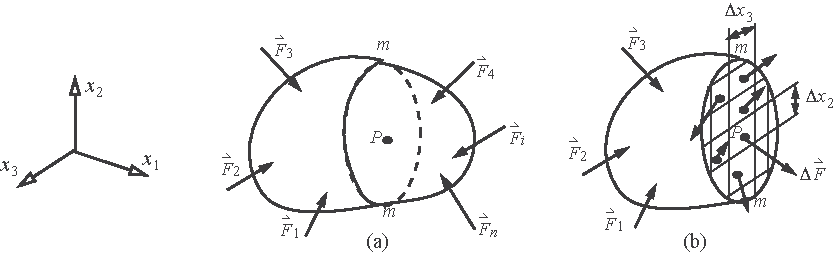
\includegraphics{Figure_A-3.pdf}
}{\caption{(a) Isolated, continuous body acted on by external forces. (b) Internal forces acting on plane~\textit{mm}.\label{figA.3}}}

Consider a continuous deformable body acted on by external forces as shown in figure~\ref{figA.3}(a). Due to the action of the external forces there will be internal forces acting between particles of the body. To examine the internal forces we pass a plane labeled \textit{mm} through point $P$ that is parallel to the $x_{2} x_{3}$ plane. Consider the free body to the left of the plane \textit{mm} shown in figure~\ref{figA.3}(b). Plane \textit{mm} is divided into a large number of small areas, each $\Delta x_{2}$ by $\Delta x_{3}$. The internal forces acting on each of these areas varies in magnitude and in direction.

 The internal force $\Delta \harp{F}$ acting at point $P$ is a resultant of distributed force intensities acting over the area $\Delta x_{2} \Delta x_{3}$. Let $\Delta A_{1}$ denote the area $\Delta x_{2} \Delta x_{3}$. Force $\Delta \harp{F}$ represents the action exerted by the material outside the plane \textit{mm} through area $\Delta A_{1}$ on the material inside the plane \textit{mm}. Point forces do not occur in nature. Forces are always distributed throughout regions, which can have dimensions of length, area, or volume. (However, point forces are an essential concept in the mechanics of solid bodies.) Consequently, as $\Delta A_{1} \rightarrow 0$ the resultant of the distributed force intensities acting over $\Delta A_{1}$ vanishes (i.e, $\Delta \harp{F} \rightarrow 0$). The stress vector or traction vector acting at point $P$ is defined as\vspace*{-9pt}
\begin{align}\label{eqA.67}
\harp{T}^{(\hat{i}_{1})}= \lim_{\Delta A_{1} \rightarrow\,0}(\Delta \harp{F} / \Delta A_{1}),
\end{align}

\vspace*{-1.2pc}

\noindent where the unit normal to area $\Delta A_{1}$ is $\hat{i}_{1}$. Now consider a rectangular parallelepiped with edges $\Delta x_{1}$, $\Delta x_{2}$, and $\Delta x_{3}$ cut out of the body. It will have six separate plane surfaces, which enclose the volume containing point $P$. Identify a surface face in terms of the coordinate axis normal to the surface. A face is defined as a positive face when its outwardly directed normal vector points in the direction of the positive coordinate direction, and as a negative face when its outward normal vector points in the negative coordinate direction. The projection of the parallelepiped in the $x_{1}$-$x_{2}$ plane is shown figure~\ref{figA.4}, where only the internal forces acting on the positive and negative faces normal to the $x_{1}$-axis are explicitly shown. Not shown in the figure are the surface forces acting on the four lateral faces and the body force acting on the volume. Let $\Delta x_{1} \rightarrow 0$ without changing the values of $\Delta x_{2}$ and $\Delta x_{3}$. In the limit the forces acting on the lateral surfaces and the body force vanish, and force equilibrium yields
\begin{wrapfigure}[12]{l}{164pt}
%\vspace{-19pt}
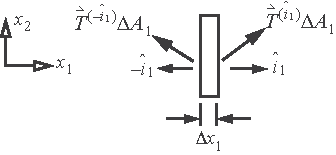
\includegraphics{Figure_A-4.pdf}
\caption{Tractions acting on the positive $x_{\textbf{1}}$-face and negative $x_{\textbf{1}}$-face of a narrow width parallelepiped.\label{figA.4}}
\end{wrapfigure}
\vspace*{-1pc}
%\vspace*{-1\baselineskip}
\begin{align}\label{eqA.68}
\harp{T}^{(-\hat{i}_{1})} \Delta A_{1}+\harp{T}^{(\hat{i}_{1})} \Delta A_{1}=0.
\end{align}
Since $\Delta A_{1}>0$, we find from equilibrium that the stress vector on the negative $x_{1}$-face is equal to the negative of the stress vector on the positive $x_{1}$-face; i.e.,
\begin{align}\label{eqA.69}
\harp{T}^{(-\hat{i}_{1})}=-\harp{T}^{(\hat{i}_{1})}.
\end{align}
 To simplify the notation let $\harp{T}_{1}=\harp{T}^{(\hat{i}_{1})}$. Stress vectors acting on the positive $x_{2}$-face and the positive $x_{3}$-face are denoted by $\harp{T}_{2}=\harp{T}^{(\hat{i}_{2})}$ and $\harp{T}_{3}=\harp{T}^{(\hat{i}_{3})}$, respectively. Stress vectors acting on the negative $x_{2}$-face and the negative $x_{3}$-face are denoted by $-\harp{T}_{2}$ and $-\harp{T}_{3}$, respectively.

Define the stress components $\sigma_{i j}=\harp{T}_{i} \bullet \hat{i}_{j}$, $i, j=1,2,3$. The first subscript on $\sigma_{i j}$ is associated with the direction normal to the face, and the second subscript is associated with the direction of the stress component. Thus\break the stress vectors in terms of components are
\begin{align}\label{eqA.70}
\begin{aligned}
&\harp{T}_{1}=\sigma_{11} \hat{i}_{1}+\sigma_{12} \hat{i}_{2}+\sigma_{13} \hat{i}_{3} \\
&\harp{T}_{2}=\sigma_{21} \hat{i}_{1}+\sigma_{22} \hat{i}_{2}+\sigma_{23} \hat{i}_{3} \\
&\harp{T}_{3}=\sigma_{31} \hat{i}_{1}+\sigma_{32} \hat{l}_{2}+\sigma_{33} \hat{l}_{3}
\end{aligned}\mbox{ or equivalently }
\left[\begin{array}{@{}c@{}}\harp{T}_{1} \\[4pt] \harp{T}_{2} \\[4pt] \harp{T}_{3}\end{array}\right]=\left[\begin{array}{@{}lll@{}}\sigma_{11} & \sigma_{12} & \sigma_{13} \\\sigma_{21} & \sigma_{22} & \sigma_{23} \\\sigma_{31} & \sigma_{32} & \sigma_{33}\end{array}\right]\left[\begin{array}{@{}l@{}}\hat{l}_{1} \\\hat{i}_{2} \\\hat{i}_{3}\end{array}\right]\!.
\end{align}
\noindent Positive stress components acting on the positive faces of the rectangular parallelepiped are shown in figure~\ref{figA.5}. The stress components on the negative faces of the parallelepiped are equal and oppositely directed to those on the positive faces according to conditions like eq. (\ref{eqA.69}). Hence, there are nine stress components at a point, not eighteen. We express the nine stress components at a point in the matrix form%\vspace*{-2pt}
\begin{align}\label{eqA.71}
[\sigma]=\left[\begin{array}{@{}lll@{}}\sigma_{11} & \sigma_{12} & \sigma_{13} \\\sigma_{21} & \sigma_{22} & \sigma_{23} \\\sigma_{31} & \sigma_{32} & \sigma_{33}\end{array}\right].
\end{align}

\vspace*{-1pc}

\noindent The diagonal elements in the stress matrix (\ref{eqA.71}) are the normal stresses, and the off-diagonal elements are the shear stresses. The nine stresses in matrix (\ref{eqA.71}) are shown in figure~\ref{figA.5}.\vspace*{-3pt}
\processfigure{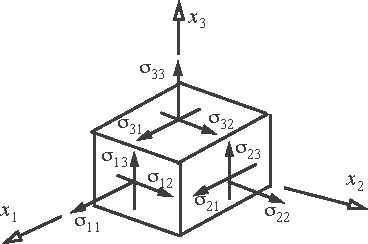
\includegraphics{Figure_A-5.pdf}
}{\caption{Stresses acting on the positive coordinate faces of a rectangular parallelepiped.\label{figA.5}}}
\processfigure[b]{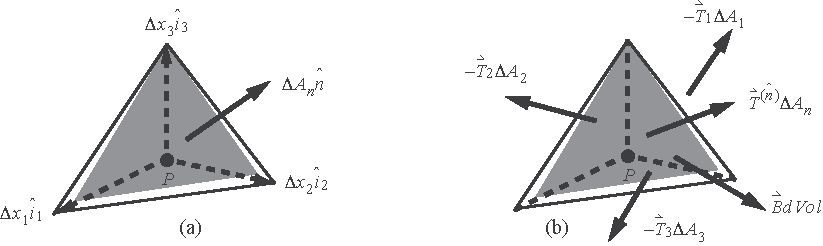
\includegraphics{Figure_A-6.pdf}
}{\caption{(a) Geometry of the tetrahedron at point $P$. (b) Free body diagram of the tetrahedron.\label{figA.6}}}

\vspace*{-7pt}

We pose the following question: Are the nine stress components at point $P$ sufficient to determine the stresses on an arbitrarily orientated plane face through the point? To answer this question we consider equilibrium of a tetrahedron cut from the body at point $P$.  The external surfaces of the tetrahedron shown in figure~\ref{figA.6}(a) consist of three right triangles normal to the coordinate axes, and one oblique triangular area that is shaded in figure~\ref{figA.6}. For the surface with unit outward normal vector $-\hat{i}_{1}$, the area is $\Delta A_{1}=(\Delta x_{2} \Delta x_{3}) / 2$; for the surface with unit\vadjust{\pagebreak} outward normal $-\hat{i}_{2}$, the area is $\Delta A_{2}=(\Delta x_{1} \Delta x_{3}) / 2$; and for the surface with unit outward normal vector $-\hat{i}_{3}$ the area is $\Delta A_{3}=(\Delta x_{1} \Delta x_{2}) / 2$. The area of the oblique surface is denoted by $\Delta A_{n}$, and its unit outward normal vector is $\hat{n}$. To calculate the area of the oblique face we use the fact that the cross product of two position vectors is equal to the area of a parallelogram formed by the vectors and in a direction normal to the plane of the parallelogram. Two of the vectors along the edges of the oblique face are $-\Delta x_{1} \hat{i}_{1}+\Delta x_{2} \hat{i}_{2}$ and $-\Delta x_{1} \hat{i}_{1}+\Delta x_{3} \hat{i}_{3}$, and the area of the parallelogram formed by these vectors is equal to $2 A_{n}$. Thus,
\begin{align}\label{eqA.72}
2 \Delta A_{n} \hat{n}=\big(-\Delta x_{1} \hat{i}_{1}+\Delta x_{2} \hat{i}_{2}\big) \times\big(-\Delta x_{1} \hat{i}_{1}+\Delta x_{3} \hat{i}_{3}\big)=\big(\Delta x_{2} \Delta x_{3} \hat{i}_{1}+\Delta x_{1} \Delta x_{3} \hat{i}_{2}+\Delta x_{1} \Delta x_{2} \hat{i}_{3}\big),
\end{align}
which simplifies to
\begin{align}\label{eqA.73}
\Delta A_{n} \hat{n}=\Delta A_{1} \hat{i}_{1}+\Delta A_{2} \hat{i}_{2}+\Delta A_{3} \hat{i}_{3}.
\end{align}
From eq. (\ref{eqA.73}) we find that area of the oblique face $\Delta A_{n}=\sqrt{(\Delta A_{1})^{2}+(\Delta A_{2})^{2}+(\Delta A_{3})^{2}}$, and the components of the unit normal vector are
\begin{align}\label{eqA.74}
n_{1}=\Delta A_{1} / \Delta A_{n} \quad n_{2}=\Delta A_{2} / \Delta A_{n} \quad n_{3}=\Delta A_{3} / \Delta A_{n}.
\end{align}
Equilibrium of the free body diagram in figure~\ref{figA.6}(b) leads to
\begin{align}\label{eqA.75}
\harp{T}^{(\hat{n})} \Delta A_{n}+\left(-\harp{T}_{1} \Delta A_{1}\right)+\left(-\harp{T}_{2} \Delta A_{2}\right)+\left(-\harp{T}_{3} \Delta A_{3}\right)+\harp{B}(d V o l)=0,
\end{align}
where $\harp{B}$ is the body force vector per unit volume. The tetrahedron is also a triangular pyramid where $\Delta A_{n}$ is the area of its triangular base, and the volume of the pyramid is $h \Delta A_{n} / 3$ where $h$ is its height. Divide eq. (\ref{eqA.75}) by $\Delta A_{n}$ to get
\begin{align}\label{eqA.76}
\harp{T}^{(n)}=\harp{T}_{1} n_{1}+\harp{T}_{2} n_{2}+\harp{T}_{3} n_{3}-\harp{B}(h / 3).
\end{align}
It can be shown that the height in this case is given by $h=\Delta x_{1} n_{1}=\Delta x_{2} n_{2}=\Delta x_{3} n_{3}$. In the limit where $\Delta x_{1} \rightarrow 0$, $\Delta x_{2} \rightarrow 0$ and $\Delta x_{3} \rightarrow 0$, the height $h \rightarrow 0$. Hence, in the limit the equilibrium equation is
\begin{align}\label{eqA.77}
\harp{T}^{(\hat{n})}=\harp{T}_{1} n_{1}+\harp{T}_{2} n_{2}+\harp{T}_{3} n_{3}.
\end{align}
The implication of eq. (\ref{eqA.77}) is that the nine stress components $\sigma_{i j}$ at point $P$ are sufficient to determine the traction, or stresses, on any face through the point.


\subsection{Equilibrium differential equations}\label{secA.2.1}

Consider the forces acting on a rectangular parallelepiped at point $P$. The free body diagram is shown in figure~\ref{figA.7}.  The vector sum of forces is
\processfigure{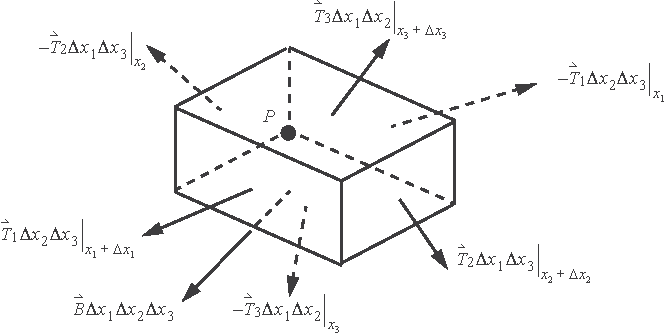
\includegraphics{Figure_A-7.pdf}
}{\caption{Surface\break forces and a body force acting on~a~rectan\-gular~parallelepiped $\Delta x_{\textbf{1}}\Delta x_{\textbf{2}}\Delta x_{\textbf{3}}$.\label{figA.7}}}
\begin{align*}
&\harp{T}_{1} \Delta x_{2} \Delta x_{3}\big|_{x_{1} +\Delta x_{1}}-\harp{T}_{1} \Delta x_{2} \Delta x_{3}\big|_{x_{1}}+\harp{T}_{2} \Delta x_{1} \Delta x_{3}\big|_{x_{2}+\Delta x_{2}}-\harp{T}_{2} \Delta x_{1} \Delta x_{3}\big|_{x_{2}}+\harp{T}_{3} \Delta x_{1} \Delta x_{2}\big|_{x_{3}+\Delta x_{3}}\\
&\quad-\harp{T}_{3} \Delta x_{1} \Delta x_{2}\big|_{x_{3}}+\harp{B} \Delta x_{1} \Delta x_{2} \Delta x_{3}.
\end{align*}
For small increments in $\Delta x_{i}$, $i=1,2,3$, use the Taylor series representation of surface forces results in the~equil\-ibrium equation to get eq. (\ref{eqA.78}) below.
\begin{align}\label{eqA.78}
\frac{\partial}{\partial x_{1}}\left(\harp{T}_{1} \Delta x_{2} \Delta x_{3}\right) \Delta x_{1}+\frac{\partial}{\partial x_{2}}\left(\harp{T}_{2} \Delta x_{1} \Delta x_{3}\right) \Delta x_{2}+\frac{\partial}{\partial x_{3}}\left(\harp{T}_{3} \Delta x_{1} \Delta x_{2}\right) \Delta x_{3}+\harp{B} \Delta x_{1} \Delta x_{2} \Delta x_{3}+O\big((\Delta x_{i})^{4}\big)=0.
\end{align}
Arrange the terms in eq. (\ref{eqA.78}) to the form
\begin{align}\label{eqA.79}
\left(\frac{\partial \harp{T}_{1}}{\partial x_{1}}+\frac{\partial \harp{T}_{2}}{\partial x_{2}}+\frac{\partial \harp{T}_{3}}{\partial x_{3}}+\harp{B}\right) \Delta x_{1} \Delta x_{2} \Delta x_{3}+O\big((\Delta x_{i})^{4}\big)=0
\end{align}
Divide eq. (\ref{eqA.79}) by the volume followed by the limit as $\Delta x_{1} \Delta x_{2} \Delta x_{3} \rightarrow 0$ to get the vector differential equation of force equilibrium at point $P$ as
\begin{align}\label{eqA.80}
\frac{\partial \harp{T}_{1}}{\partial x_{1}}+\frac{\partial \harp{T}_{2}}{\partial x_{2}}+\frac{\partial \harp{T}_{3}}{\partial x_{3}}+\harp{B}=0.
\end{align}
Substitute eq. (\ref{eqA.70}) for the traction vectors in eq. (\ref{eqA.80}) to write the equilibrium differential equations in the $x_{i}$-coordinate directions. In the order of $x_{1}$, $x_{2}$, $x_{3}$ coordinate directions these equations are
\begin{align}\label{eqA.81}	
\begin{aligned}
&\frac{\partial \sigma_{11}}{\partial x_{1}}+\frac{\partial \sigma_{21}}{\partial x_{2}}+\frac{\partial \sigma_{31}}{\partial x_{3}}+B_{1}=0\\ &\frac{\partial \sigma_{12}}{\partial x_{1}}+\frac{\partial \sigma_{22}}{\partial x_{2}}+\frac{\partial \sigma_{32}}{\partial x_{3}}+B_{2}=0\\ &\frac{\partial \sigma_{13}}{\partial x_{1}}+\frac{\partial \sigma_{23}}{\partial x_{2}}+\frac{\partial \sigma_{33}}{\partial x_{3}}+B_{3}=0\end{aligned}.
\end{align}\processfigure{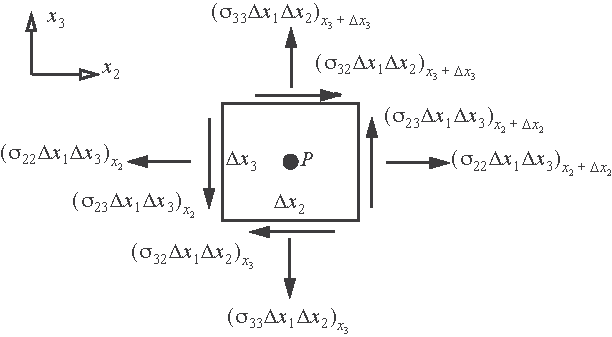
\includegraphics{Figure_A-8.pdf}
}{\caption{A free body diagram of the parallelepiped at point $P$ for moment equilibrium about the $x_{\textbf{1}}$-axis. The $x_{\textbf{1}}$-axis points normal to the page toward the reader.\label{figA.8}}}\noindent Now consider moment equilibrium about the coordinate axes of the rectangular parallelepiped at point $P$. For moment equilibrium about the $x_{1}$-axis refer to the free body diagram in figure~\ref{figA.8}.  The moment arm from point $P$ to the line of action of the normal force $(\sigma_{22} \Delta x_{1} \Delta x_{3})_{x_{2}+\Delta x_{2}}$ acting on the positive $x_{2}$-face is denoted by $\varepsilon \Delta x_{3}$, where $\varepsilon$ is a small numerical value. Parameter $\varepsilon$ is not known, but this will not matter in the end result. The moment arm from point $P$ to the line of action of the shear force $(\sigma_{23} \Delta x_{1} \Delta x_{3})_{x_{2}+\Delta x_{2}}$ acting on the positive $x_{2}$ face is $\Delta x_{2} / 2$. Including all the forces shown in figure~\ref{figA.8}, the sum of moments about the $x_{1}$-axis through point $P$, counterclockwise positive, is
\begin{align}\label{eqA.82}
&-\varepsilon \Delta x_{3}(\sigma_{22} \Delta x_{1} \Delta x_{3})_{x_{2}+\Delta x_{2}}+\varepsilon \Delta x_{3}(\sigma_{22} \Delta x_{1} \Delta x_{3})_{x_{2}}+\frac{\Delta x_{2}}{2}(\sigma_{23} \Delta x_{1} \Delta x_{3})_{x_{2}+\Delta x_{2}}+\frac{\Delta x_{2}}{2}(\sigma_{23} \Delta x_{1} \Delta x_{3})_{x_{2}}\nonumber\\
&\quad+\varepsilon \Delta x_{2}(\sigma_{33} \Delta x_{1} \Delta x_{2})_{x_{3}+\Delta x_{3}}-\varepsilon \Delta_{2}(\sigma_{33} \Delta x_{1} \Delta x_{2})_{x_{3}}-\frac{\Delta x_{3}}{2}(\sigma_{32} \Delta x_{1} \Delta x_{2})_{x_{3}+\Delta x_{3}}-\frac{\Delta x_{3}}{2}(\sigma_{32} \Delta x_{1} \Delta x_{2})_{x_{3}}=0.
\end{align}

\pagebreak
\noindent Use the Taylor series to expand the forces acting on the positive coordinate faces with respect to the forces acting on the negative coordinate faces to get
\begin{align}\label{eqA.83}
&-\varepsilon \Delta x_{3}\left[\frac{\partial \sigma_{22}}{\partial x_{2}} \Delta x_{2}+O(\Delta x_{2}^{2})\right] \Delta x_{1} \Delta x_{3}+\frac{\Delta x_{2}}{2}\left[2 \sigma_{23}+\frac{\partial \sigma_{23}}{\partial x_{2}} \Delta x_{2}+O(\Delta x_{2}^{2})\right] \Delta x_{1} \Delta x_{3}\nonumber\\
&\quad+\varepsilon \Delta x_{2}\left[\frac{\partial \sigma_{33}}{\partial x_{3}} \Delta x_{3}+O(\Delta x_{3}^{2})\right] \Delta x_{1} \Delta x_{2}-\frac{\Delta x_{3}}{2}\left[2 \sigma_{32}+\frac{\partial \sigma_{32}}{\partial x_{3}} \Delta x_{3}+O(\Delta x_{3}^{2})\right] \Delta x_{1} \Delta x_{2}=0.
\end{align}
Expand eq. (\ref{eqA.83}) in powers of $\Delta x_{i}$ to write it as
\begin{align}\label{eqA.84}
\left(\sigma_{23}-\sigma_{32}\right) \Delta x_{1} \Delta x_{2} \Delta x_{3}+\varepsilon\left[-\frac{\partial \sigma_{22}}{\partial x_{2}} \Delta x_{1} \Delta x_{2} \Delta x_{3}^{2}+\frac{\partial \sigma_{33}}{\partial x_{3}} \Delta x_{1} \Delta x_{2}^{2} \Delta x_{3}\right]+\text { H.O.T. }=0,
\end{align}
where H.O.T. means higher order terms, that is, terms of quartic powers and higher in the increments in the coordinates. Notice the terms multiplied by $\varepsilon$ are quartic powers of the increments in the coordinates. Division of eq. (\ref{eqA.84}) by $\Delta x_{1} \Delta x_{2} \Delta x_{3}$, followed by the limit of $\Delta x_{i} \rightarrow 0$ leads the condition of moment equilibrium about the $x_{1}$-axis that $\sigma_{23}-\sigma_{32}=0$. Moment equilibrium about the $x_{2}$-axis leads to $\sigma_{31}-\sigma_{13}=0$, and moment equilibrium about the $x_{3}$-axis leads to $\sigma_{12}-\sigma_{21}=0$. The equations of moment equilibrium at point $P$ are
\begin{align}\label{eqA.85}
\sigma_{12}=\sigma_{21} \quad \sigma_{13}=\sigma_{31} \quad \sigma_{23}=\sigma_{32}.
\end{align}
Hence, the stress matrix (\ref{eqA.71}) is symmetric.

\subsection{Transformation of stresses between two Cartesian coordinate systems}\label{secA.2.2}

At point $P$ coordinates $(x_{1}^{\prime}, x_{2}^{\prime}, x_{3}^{\prime})$ are linearly related to coordinates $(x_{1}, x_{2}, x_{3})$ by eq. (\ref{eqA.41}). The stress components $\sigma_{i j}$ are functions in the variables $(x_{1}, x_{2}, x_{3})$, and the stresses $\sigma_{i j}^{\prime}$ are functions in the variables\break $(x_{1}^{\prime}, x_{2}^{\prime}, x_{3}^{\prime})$. The~stress vectors acting on the $x_{i}$-faces are denoted by $\harp{T}_{i}$, and those acting on the $x_{i}^{\prime}$-faces are denoted by $\harp{T}_{i}^{\prime}$.~These stress vectors are written in their respective coordinate systems by
\begin{align}\label{eqA.86}
\left[\begin{array}{@{}c@{}}\harp{T}_{1} \\[4pt] \harp{T}_{2} \\[4pt] \harp{T}_{3}\end{array}\right]=\left[\begin{array}{@{}lll@{}}\sigma_{11} & \sigma_{12} & \sigma_{13} \\\sigma_{21} & \sigma_{22} & \sigma_{23} \\\sigma_{31} & \sigma_{32} & \sigma_{33}\end{array}\right]\left[\begin{array}{@{}l@{}}\hat{i}_{1} \\[4pt] \hat{i}_{2} \\[4pt] \hat{i}_{3}\end{array}\right]\mbox{, and } \left[\begin{array}{@{}c@{}}\harp{T}_{1}^{\prime} \\[4pt] \harp{T}_{2}^{\prime} \\[4pt] \harp{T}_{3}^{\prime}\end{array}\right]=
\left[\begin{array}{@{}lll@{}}\sigma_{11}^{\prime} & \sigma_{12}^{\prime} & \sigma_{13}^{\prime} \\[4pt]\sigma_{21}^{\prime} & \sigma_{22}^{\prime} & \sigma_{23}^{\prime} \\[4pt]\sigma_{31}^{\prime} & \sigma_{32}^{\prime} & \sigma_{33}^{\prime}\end{array}\right]\left[\begin{array}{@{}l@{}}\hat{i}_{1}^{\,\prime} \\[4pt] \hat{i}_{2}^{\,\prime} \\[4pt] \hat{i}_{3}^{\,\prime}\end{array}\right]\!.
\end{align}
In eq. (\ref{eqA.86}) the stress matrices are
\begin{align}\label{eqA.87}
[\sigma]=\left[\begin{array}{@{}lll@{}}\sigma_{11} & \sigma_{12} & \sigma_{13} \\\sigma_{21} & \sigma_{22} & \sigma_{23} \\\sigma_{31} & \sigma_{32} & \sigma_{33}\end{array}\right]\mbox{, and }[\sigma^{\prime}]=\left[\begin{array}{@{}lll@{}}\sigma_{11}^{\prime} & \sigma_{12}^{\prime} & \sigma_{13}^{\prime} \\[4pt]\sigma_{21}^{\prime} & \sigma_{22}^{\prime} & \sigma_{23}^{\prime} \\[4pt]\sigma_{31}^{\prime} & \sigma_{32}^{\prime} & \sigma_{33}^{\prime}\end{array}\right].
\end{align}
Note that the stress matrix $[\sigma]$ is symmetric by eq. (\ref{eqA.85}). The stress transformation equations between the Cartesian coordinate systems $(x_{1}, x_{2}, x_{3})$ and $(x_{1}^{\prime}, x_{2}^{\prime}, x_{3}^{\prime})$ are determined by selecting the unit normal in eq. (\ref{eqA.77}) to be either $\hat{i}_1^{\,\prime}$, $\hat{i}_2^{\,\prime}$, or $\hat{i}_{3}^{\,\prime}$. First let $\hat{n}=\hat{i}_{1}^{\,\prime}$ such that $\harp{T}^{(n)}=\harp{T}_{1}^{\prime}$ in eq. (\ref{eqA.77}). From eq. (\ref{eqA.44}) we have $\hat{n}=\lambda_{11} \hat{i}_{1}+\lambda_{12} \hat{i}_{2}+\lambda_{13} \hat{i}_{3}$. Hence, eq. (\ref{eqA.77}) becomes
\begin{align}\label{eqA.88}
\harp{T}_{1}^{\prime}=\lambda_{11} \harp{T}_{1}+\lambda_{12} \harp{T}_{2}+\lambda_{13} \harp{T}_{3}.
\end{align}
Second, let $\hat{n}=\hat{i}_{2}^{\,\prime}$ such that $\harp{T}^{(n)}=\harp{T}_{2}^{\prime}$. From eq. (\ref{eqA.44}) we have $\hat{n}=\lambda_{21} \hat{i}_{1}+\lambda_{22} \hat{i}_{2}+\lambda_{23} \hat{i}_{3}$. Hence, eq. (\ref{eqA.77}) becomes
\begin{align}\label{eqA.89}
\harp{T}_{2}^{\prime}=\lambda_{21} \harp{T}_{1}+\lambda_{22} \harp{T}_{2}+\lambda_{23} \harp{T}_{3}.
\end{align}
Third, let $\hat{n}=\hat{i}_{3}^{\,\prime}$ that $\harp{T}^{(n)}=\harp{T}_{3}^{\prime}$ and $\hat{n}=\lambda_{31} \hat{i}_{1}+\lambda_{32} \hat{i}_{2}+\lambda_{33} \hat{i}_{3}$. Hence,
\begin{align}\label{eqA.90}
\harp{T}_{3}^{\prime}=\lambda_{31} \harp{T}_{1}+\lambda_{32} \harp{T}_{2}+\lambda_{33} \harp{T}_{3}.
\end{align}
The three selections for the unit normal in eq. (\ref{eqA.77}) relate the tractions acting on the $x_{i}^{\prime}$ coordinate faces to the tractions acting on the $x_{i}$-faces by
\begin{align}\label{eqA.91}
\left[\begin{array}{@{}c@{}}\harp{T}_{1}^{\prime} \\[4pt] \harp{T}_{2}^{\prime} \\[4pt] \harp{T}_{3}^{\prime}\end{array}\right]=\left[\begin{array}{@{}lll@{}}\lambda_{11} & \lambda_{12} & \lambda_{13} \\\lambda_{21} & \lambda_{22} & \lambda_{23} \\\lambda_{31} & \lambda_{32} & \lambda_{33}\end{array}\right]\left[\begin{array}{@{}c@{}}\harp{T}_{1} \\[4pt] \harp{T}_{2} \\[4pt] \harp{T}_{3}\end{array}\right].
\end{align}
Substitute the expressions for the stress vectors from eq. (\ref{eqA.86}) into eq. (\ref{eqA.91}) to get
\begin{align}\label{eqA.92}
\left[\begin{array}{@{}lll@{}}
\sigma_{11}^{\prime} & \sigma_{12}^{\prime} & \sigma_{13} \\[5pt]
\sigma_{21}^{\prime} & \sigma_{22}^{\prime} & \sigma_{23} \\[5pt]
\sigma_{31}^{\prime} & \sigma_{32}^{\prime} & \sigma_{33}\end{array}\right]\left[\begin{array}{@{}l@{}}\hat{i}_{1}^{\,\prime} \\[4pt] \hat{i}_{2}^{\,\prime} \\[4pt] \hat{i}_{3}^{\,\prime}\end{array}\right]=\left[\begin{array}{@{}lll@{}}\lambda_{11} & \lambda_{12} & \lambda_{13} \\\lambda_{21} & \lambda_{22} & \lambda_{23} \\\lambda_{31} & \lambda_{32} & \lambda_{33}\end{array}\right]\left[\begin{array}{@{}lll@{}}\sigma_{11} & \sigma_{12} & \sigma_{13} \\\sigma_{21} & \sigma_{22} & \sigma_{23} \\\sigma_{31} & \sigma_{32} & \sigma_{33}\end{array}\right]\left[\begin{array}{@{}l@{}}\hat{i}_{1} \\[4pt] \hat{i}_{2} \\[4pt] \hat{i}_{3}\end{array}\right].
\end{align}
The inverse eq. (\ref{eqA.44}) is
\begin{align}\label{eqA.93}
\left[\begin{array}{@{}l@{}}\hat{i}_{1} \\[4pt] \hat{i}_{2} \\[4pt] \hat{i}_{3}\end{array}\right]=\left[\begin{array}{@{}lll@{}}\lambda_{11} & \lambda_{21} & \lambda_{31} \\\lambda_{12} & \lambda_{22} & \lambda_{32} \\\lambda_{13} & \lambda_{23} & \lambda_{33}\end{array}\right]\left[\begin{array}{@{}l@{}}\hat{i}_{1}^{\,\prime} \\[4pt] \hat{i}_{2}^{\,\prime} \\[4pt] \hat{i}_{3}^{\,\prime}\end{array}\right].
\end{align}
Substitute eq. (\ref{eqA.93}) into the right-hand side of eq. (\ref{eqA.92}) and rearrange the result to find
\begin{align}\label{eqA.94}
\left(\left[\begin{array}{ccc}
\sigma_{11}^{\prime} & \sigma_{12}^{\prime} & \sigma_{13}^{\prime} \\[5pt]\sigma_{21}^{\prime} & \sigma_{22}^{\prime} & \sigma_{23}^{\prime} \\[5pt]\sigma_{31}^{\prime} & \sigma_{32}^{\prime} & \sigma_{33}^{\prime}\end{array}\right]-\left[\begin{array}{@{}lll@{}}\lambda_{11} & \lambda_{12} & \lambda_{13} \\\lambda_{21} & \lambda_{22} & \lambda_{23} \\\lambda_{31} & \lambda_{32} & \lambda_{33}\end{array}\right]\left[\begin{array}{@{}lll@{}}\sigma_{11} & \sigma_{12} & \sigma_{13} \\\sigma_{21} & \sigma_{22} & \sigma_{23} \\\sigma_{31} & \sigma_{32} & \sigma_{33}\end{array}\right]\left[\begin{array}{@{}lll@{}}\lambda_{11} & \lambda_{21} & \lambda_{31} \\\lambda_{12} & \lambda_{22} & \lambda_{32} \\\lambda_{13} & \lambda_{23} & \lambda_{33}\end{array}\right]\right)\left[\begin{array}{@{}l@{}}\hat{i}_{1}^{\,\prime} \\[4pt] \hat{i}_{2}^{\,\prime} \\[4pt] \hat{i}_{3}^{\,\prime}\end{array}\right]=\left[\begin{array}{@{}l@{}}0 \\0 \\0\end{array}\right].
\end{align}
To satisfy eq. (\ref{eqA.94}) we find that the stress components $\sigma_{i j}^{\prime}$ in the $x_{i}^{\prime}$-system are related to the stress components $\sigma_{i j}$ in the $x_{i}$-system by
\begin{align}\label{eqA.95}
\left[\begin{array}{@{}lll@{}}\sigma_{11}^{\prime} & \sigma_{12}^{\prime} & \sigma_{13} \\[3pt]
\sigma_{21}^{\prime} & \sigma_{22}^{\prime} & \sigma_{23}^{\prime} \\[3pt]
\sigma_{31}^{\prime} & \sigma_{32}^{\prime} & \sigma_{33}^{\prime}\end{array}\right]=\left[\begin{array}{@{}lll@{}}\lambda_{11} & \lambda_{12} & \lambda_{13} \\\lambda_{21} & \lambda_{22} & \lambda_{23} \\\lambda_{31} & \lambda_{32} & \lambda_{33}\end{array}\right]\left[\begin{array}{@{}lll@{}}\sigma_{11} & \sigma_{12} & \sigma_{13} \\\sigma_{21} & \sigma_{22} & \sigma_{23} \\\sigma_{31} & \sigma_{32} & \sigma_{33}\end{array}\right]\left[\begin{array}{@{}lll@{}}\lambda_{11} & \lambda_{21} & \lambda_{31} \\\lambda_{12} & \lambda_{22} & \lambda_{32} \\\lambda_{13} & \lambda_{23} & \lambda_{33}\end{array}\right].
\end{align}
Equation (\ref{eqA.95}) in compact form is
\begin{align}\label{eqA.96}
[\sigma^{\prime}]=[\lambda][\sigma][\lambda]^{T}.
\end{align}
Pre-multiply eq. (\ref{eqA.96}) by $[\lambda]^{T}$, post-multiply it by $[\lambda]$, and note that $[\lambda]^{T}[\lambda]=[\lambda][\lambda]^{T}=[I]$ to find the inverse transformation
\begin{align}\label{eqA.97}
[\sigma]=[\lambda]^{T}[\sigma^{\prime}][\lambda].
\end{align}
The transpose of eq. (\ref{eqA.96}) is $[\lambda][\sigma]^{T}[\lambda]^{T}$, but $[\sigma]^{T}=[\sigma]$, so the stress matrix $[\sigma^{\prime}]$ is also symmetric. Comparing the strain transformation eq. (\ref{eqA.63}) to the stress transformation eq. (\ref{eqA.96}), it is clear that the transformation of strains $\varepsilon_{ij}$ is the same form as the transformation of the stresses $\sigma_{ij}$.

\subsection{Cartesian tensors}\label{secA.2.3}

A \textbf{tensor} is a system of numbers or functions, whose components obey a certain law of transformation when the independent variables undergo a linear transformation. If the independent variables are the rectangular cartesian systems $x_{i}$ and $x_{i}^{\prime}$ transforming by the linear relations given by $\{x^{\prime}\}=[\lambda]\{x\}$ at point $P$, then the systems obeying certain laws of transformation are called Cartesian tensors.

\smallskip\vspace*{-2pt}%\bigskip

\noindent\textbf{Definition.}\enspace A system of order two may be defined to have nine components $\varepsilon_{i j}$ in $x_{i}$ and nine components $\varepsilon_{ij}^{\prime}$ in~$x_{i}^{\prime}$.~If
\begin{align}\label{eqA.98}
[\varepsilon_{i j}^{\prime}]=[\lambda][\varepsilon_{i j}][\lambda]^{T}
\end{align}
then the functions $\varepsilon_{ij}$ and $\varepsilon_{ij}^{\prime}$ are the components in their respective variables of a second order Cartesian tensor. Similarly, functions $\sigma_{ij}$ and $\sigma_{ij}^{\prime}$ are the components in their respective variables of a second order Cartesian tensor.

\section{Linear elastic material law}\label{secA.3}

To this point in the study of the mechanics of a solid body we have eighteen unknown functions of the Cartesian coordinates $x_{1}$, $x_{2}$, and $x_{3}$. These are the three displacements $u_{1}$, $u_{2}$, and $u_{3}$, the six strains $\varepsilon_{11}$, $\varepsilon_{22}$, $\varepsilon_{33}$, $\gamma_{23}$, $\gamma_{31}$, and $\gamma_{12}$, and nine stresses $\sigma_{11}$, $\sigma_{12}$, $\sigma_{13}$, $\sigma_{21}$, $\sigma_{22}$, $\sigma_{23}$, $\sigma_{31}$, $\sigma_{32}$, and $\sigma_{33}$. There are twelve equations relating these unknowns; the six strain-displacement equations (\ref{eqA.35}) and (\ref{eqA.36}), and the six equilibrium equations (\ref{eqA.81}) and (\ref{eqA.85}). Therefore we need six more equations to get the number of unknowns equal to number of equations. The additional six equations come from the relations between the strains and the stresses, which express the material law. This relation between strains and stresses for different materials is established by material characterization tests on standard test specimens.

Solid bodies that can instantly recover their original size and shape when the forces producing the deformation are removed are called perfectly elastic. The elastic limit is defined as the greatest stress that can be applied without resulting in permanent strain on release of the stress. Elasticity is applicable to any body provided the stresses do not exceed the elastic limit. For many solid bodies there is a region where the stress is very nearly proportional to strain. The proportional limit is defined as the greatest stress for which the stress is still proportional to the strain. Both the elastic limit and proportional limit cannot be precisely determined from test data since they are defined by the limiting cases of no permanent deformation and no deviation from linearity. In practice the definition of the yield strength of a material is used to determine the limit of elastic behavior. See article \ref{sec4.2} on page \pageref{sec4.2} for a discussion on yield criteria.

\subsection{First law of thermodynamics}\label{secA.3.1}

The theoretical basis for an elastic material law is the first law of thermodynamics applied to an arbitrary infinitesimal rectangular parallelepiped isolated from the body. We assume the deformation process is adiabatic. That is, no heat is lost or gained in the body during the deformation. An alternate definition of elastic behavior is that the work expended in the transition from the reference state to the final deformed state is independent of the manner in which the process proceeds. The first law of thermodynamics states that work done on the rectangular parallelepiped is equal to the change in internal energy of the material contained in the parallelepiped.\footnote{We are not considering the change in kinetic energy for simplicity. If kinetic energy were actuated for in the first law of thermodynamics, then the final results obtained in this article would be unchanged.} In elasticity the internal energy is called the strain energy. The incremental work of the tractions and body force acting on the parallelepiped are formulated in terms of incremental displacements from the equilibrium state. These incremental displacement functions are denoted by $\delta u_{i}(x_{1}, x_{2}, x_{3})$, $i=1,2,3$, and to be kinematically admissible they are continuous and single-valued in the independent variables. In addition, functions $\delta u_{i}$ are assumed to be infinitesimal in magnitude. The total displacement at point $P$ is $\tilde{u}_{i}=u_{i}+\delta u_{i}$, where $u_{i}$ are the displacements components in the equilibrium state.

\begin{wrapfigure}[14]{R}{158.14pt}
\vspace*{-19pt}
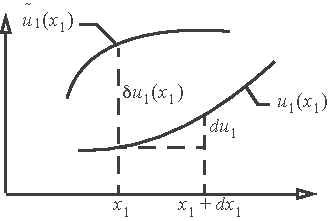
\includegraphics{Figure_A-9.pdf}
\caption{Graph of $u_{\textbf{1}}(x_{\textbf{1}})$ and $\tilde{u}_{\textbf{1}}(x_{\textbf{1}})$.\label{figA.9}}
\vspace*{-1pc}
\end{wrapfigure}

\subsubsection{The distinction between $\boldsymbol{\delta} \textbf{\textit{u}}_{\textbf{1}}$ and $\textbf{\textit{du}}_{\textbf{1}}$.} In one dimension we define $u_{1}(x_{1})$ as the displacement function of a particle originally at coordinate $x_{1}$ in the reference configuration of the body (region $B_{0}$). The definition of incremental work necessitates consideration of the incremental displacement of a particle in the body. The distinction between $\delta u_{1}$ and $d u_{1}$ is illustrated in figure~\ref{figA.9}. The incremental displacement $\delta u_{1}$ is at a fixed value of the independent variable $x_{1}$, and the differential $d u_{1}$ is the change in displacement with respect to the change in the independent variable $x_{1}$. In the formulation of incremental work we interpret $\delta u_{1}$ as the infinitesimal change in a the displacement of one particle identified by its coordinate in region $B_{0}$. The interpretation of $d u_{1}$ is the relative displacement between two particles, one originally at $x_{1}+d x_{1}$ and the other originally at $x_{1}$ in region $B_{0}$. The symbol $\delta$ is called a variational operator, and the symbol $d$ or the symbol $\partial$ are a differential operators.




For an adiabatic deformation process the first law of thermodynamics for the material in the rectangular parallelepiped of figure~\ref{figA.7} is
\begin{align}\label{eqA.99}
&\harp{T}_{1} \Delta x_{2} \Delta x_{3} \bullet \delta \harp{u}\big|_{x_{1}+\Delta x_{1}}+\left(-\harp{T}_{1} \Delta x_{2} \Delta x_{3} \bullet \delta \harp{u}\right)\big|_{x_{1}}+\harp{T}_{2} \Delta x_{1} \Delta x_{3} \bullet \delta \harp{u}\big|_{x_{2}+\Delta x_{2}}+\left(-\harp{T}_{2} \Delta x_{1} \Delta x_{3} \bullet \delta \harp{u}\right)\big|_{x_{2}}\nonumber\\
&\quad+\harp{T}_{3} \Delta x_{1} \Delta x_{2} \bullet \delta \harp{u}\big|_{x_{3}+\Delta x_{3}}+\left(-\harp{T}_{3} \Delta x_{1} \Delta x_{2} \bullet \delta \harp{u}\right)\big|_{x_{3}}+\harp{B} \Delta x_{1} \Delta x_{2} \Delta x_{3} \bullet \delta \harp{u}=\delta U \Delta x_{1} \Delta x_{2} \Delta x_{3},
\end{align}
where the variation in the displacement vector is $\delta \harp{u}=\delta u_{1} \hat{i}_{1}+\delta u_{2} \hat{i}_{2}+\delta u_{3} \hat{i}_{3}$, and the variation the strain energy per unit volume, or the strain energy density, is $\delta U$. These variations are at fixed values of the independent variables $x_{i}$. Expand the tractions acting on the faces of the rectangular parallelepiped at point $P$ in a Taylor series keeping only those terms to the first degree in the differentials $\Delta x_{i}$ to get
\begin{align}\label{eqA.100}
\frac{\partial\left(\harp{T}_{1} \bullet \delta \harp{u}\right)}{\partial x_{1}} \Delta x_{1} \Delta x_{2} \Delta x_{3}+\frac{\partial\left(\harp{T}_{2} \bullet \delta \harp{u}\right)}{\partial x_{2}} \Delta x_{1} \Delta x_{2} \Delta x_{3}+\frac{\partial\left(\harp{T}_{3} \bullet \delta \harp{u}\right)}{\partial x_{3}} \Delta x_{1} \Delta x_{2} \Delta x_{3}+\harp{B} \Delta x_{1} \Delta x_{2} \Delta x_{3}\bullet \delta \harp{u}=\delta U \Delta x_{1} \Delta x_{2} \Delta x_{3}.
\end{align}

\vspace{-9pt}\noindent Divide eq. (\ref{eqA.100}) by the volume $\Delta x_{1} \Delta x_{2} \Delta x_{3}$ to get
\begin{align}\label{eqA.101}
\left(\frac{\partial \harp{T}_{1}}{\partial x_{1}}+\frac{\partial \harp{T}_{2}}{\partial x_{2}}+\frac{\partial \harp{T}_{3}}{\partial x_{3}}+\harp{B}\right) \bullet \delta \harp{u}+\harp{T}_{1} \bullet \frac{\partial}{\partial x_{1}}(\delta \harp{u})+T_{2} \bullet \frac{\partial}{\partial x_{2}}(\delta \harp{u})+\dot{T}_{3} \bullet \frac{\partial}{\partial x_{3}}(\delta \harp{u})=\delta U.
\end{align}
The first term on the left-hand side vanishes via equilibrium eq. (\ref{eqA.80}). Hence, (\ref{eqA.101}) reduces to
\begin{align}\label{eqA.102}
\harp{T}_{1} \bullet \frac{\partial}{\partial x_{1}}(\delta \harp{u})+\harp{T}_{2} \bullet \frac{\partial}{\partial x_{2}}(\delta \harp{u})+\harp{T}_{3} \bullet \frac{\partial}{\partial x_{3}}(\delta \harp{u})=\delta U.
\end{align}
Consider the term
\begin{align}\label{eqA.103}
\harp{T}_{1} \bullet \frac{\partial}{\partial x_{1}}(\delta \harp{u})=[\sigma_{11} \hat{i}_{1}+\sigma_{12} \hat{i}_{2}+\sigma_{13} \hat{i}_{3}] \bullet\left[\frac{\partial}{\partial x_{1}}(\delta u_{1}) \hat{i}_{1}+\frac{\partial}{\partial x_{1}}(\delta u_{2}) \hat{i}_{2}+\frac{\partial}{\partial x_{1}}(\delta u_{3}) \hat{i}_{3}\right].
\end{align}
The variation in the derivative of a function is defined by
\begin{align}\label{eqA.104}
\delta\left(\frac{\partial u_{i}}{\partial x_{j}}\right) \equiv \frac{\partial \tilde{u}_{i}}{\partial x_{j}}-\frac{\partial u_{i}}{\partial x_{j}},\ i, j=1,2,3.
\end{align}
Substitute $\tilde{u}_{i}=u_{i}+\delta u_{i}$ into eq. (\ref{eqA.104}) to get
\[
\delta\left(\frac{\partial u_{i}}{\partial x_{j}}\right)=\frac{\partial}{\partial x_{j}}(u_{i}+\delta u_{i})-\frac{\partial u_{i}}{\partial x_{j}}=\frac{\partial}{\partial x_{j}}(\delta u_{i}).
\]
Hence, the variation of the derivative of a function is equal to the derivative of the variation in the function. That~is,\vspace*{-6pt}
\begin{align}\label{eqA.105}
\delta\left(\frac{\partial u_{i}}{\partial x_{j}}\right)=\frac{\partial}{\partial x_{j}}(\delta u_{i}).
\end{align}
Employing the result of eq. (\ref{eqA.105}) in eq. (\ref{eqA.103}) we write the latter as
\begin{align}\label{eqA.106}
\harp{T}_{1} \bullet \frac{\partial}{\partial x_{1}}(\delta \harp{u}) &=\left[\sigma_{11} \hat{i}_{1}+\sigma_{12} \hat{i}_{2}+\sigma_{13} \hat{i}_{3}\right] \bullet\left[\delta\left(\frac{\partial u_{1}}{\partial x_{1}}\right) \hat{i}_{1}+\delta\left(\frac{\partial u_{2}}{\partial x_{1}}\right) \hat{i}_{2}+\delta\left(\frac{\partial u_{3}}{\partial x_{1}}\right) \hat{i}_{3}\right] \nonumber\\
&=\sigma_{11} \delta\left(\frac{\partial u_{1}}{\partial x_{1}}\right)+\sigma_{12} \delta\left(\frac{\partial u_{2}}{\partial x_{1}}\right)+\sigma_{13} \delta\left(\frac{\partial u_{3}}{\partial x_{1}}\right).
\end{align}
Similarly the remaining terms on the left-hand side of eq. (\ref{eqA.102}) can be evaluated as was done starting with eq. (\ref{eqA.103}). The result is
\begin{align}\label{eqA.107}
&\sigma_{11} \delta\left(\frac{\partial u_{1}}{\partial x_{1}}\right)+\sigma_{22} \delta\left(\frac{\partial u_{2}}{\partial x_{2}}\right)+\sigma_{33} \delta\left(\frac{\partial u_{3}}{\partial x_{3}}\right)\nonumber\\*
&\quad+\sigma_{23}\left[\delta\left(\frac{\partial u_{2}}{\partial x_{3}}\right)+\delta\left(\frac{\partial u_{3}}{\partial x_{2}}\right)\right]+\sigma_{31}\left[\delta\left(\frac{\partial u_{1}}{\partial x_{3}}\right)+\delta\left(\frac{\partial u_{3}}{\partial x_{1}}\right)\right]+\sigma_{12}\left[\delta\left(\frac{\partial u_{1}}{\partial x_{2}}\right)+\delta\left(\frac{\partial u_{2}}{\partial x_{1}}\right)\right]=\delta U.
\end{align}
The variations in the strains are determined from the linear strain-displacement relations (\ref{eqA.35}) and (\ref{eqA.36}) by letting $u_{i} \rightarrow u_{i}+\delta u_{i}$, The variations in the strains are
\[
\delta \varepsilon_{11}=\delta \frac{\partial u_{1}}{\partial x_{1}} \quad \delta \varepsilon_{22}=\delta\left(\frac{\partial u_{2}}{\partial x_{2}}\right) \quad \ldots \quad \delta \gamma_{12}=\delta\left(\frac{\partial u_{1}}{\partial x_{2}}\right)+\delta\left(\frac{\partial u_{2}}{\partial x_{1}}\right)
\]
Thus eq. (\ref{eqA.107}) is
\begin{align}\label{eqA.108}
\sigma_{11} \delta \varepsilon_{11}+\sigma_{22} \delta \varepsilon_{22}+\sigma_{33} \delta \varepsilon_{33}+\sigma_{23} \delta \gamma_{23}+\sigma_{31} \delta \gamma_{31}+\sigma_{12} \delta \gamma_{12}=\delta U.
\end{align}
In elasticity the strain energy density function is defined to be a function of the strain components; i.e., $U=U(\varepsilon_{11}, \varepsilon_{22}, \varepsilon_{33}, \gamma_{23}, \gamma_{31}, \gamma_{12})$. The strain energy density function depends on the physical properties of the material. The variation in the strain energy for the material in the rectangular parallelepiped as the strains are varied is determined from the series
\begin{align*}
&U\!\left(\varepsilon_{11}+\delta \varepsilon_{11}, \varepsilon_{22}+\delta \varepsilon_{22}, \ldots, \gamma_{12}+\delta \gamma_{12}\right)
=U\!\left(\varepsilon_{11}, \varepsilon_{22}, \ldots, \gamma_{12}\right)+\frac{\partial U}{\partial \varepsilon_{11}} \delta \varepsilon_{11}+\frac{\partial U}{\partial \varepsilon_{22}} \delta \varepsilon_{22}+\frac{\partial U}{\partial \varepsilon_{33}} \delta \varepsilon_{33}\\
&\quad+\cdots+\frac{\partial U}{\partial y_{12}} \delta \gamma_{12} + \text{H.O.T.},
\end{align*}
where H.O.T. are higher order terms that contain quadratic and higher powers in the varied strain components. The change in strain energy is given by
\[
\Delta U=U(\varepsilon_{11}+\delta \varepsilon_{11}, \varepsilon_{22}+\delta \varepsilon_{22}, \ldots, \gamma_{12}+\delta \gamma_{12})-U(\varepsilon_{11}, \varepsilon_{22}, \ldots, \gamma_{12})=\delta U+ \text{H.O.T.}
\]
For infinitesimal variations in the strains $\Delta U \sim \delta U$, where
\begin{align}\label{eqA.109}
\delta U=\frac{\partial U}{\partial \varepsilon_{11}} \delta \varepsilon_{11}+\frac{\partial U}{\partial \varepsilon_{22}} \delta \varepsilon_{22}+\frac{\partial U}{\partial \varepsilon_{33}} \delta \varepsilon_{33}+\frac{\partial U}{\partial \gamma_{23}} \delta \gamma_{23}+\frac{\partial U}{\partial \gamma_{31}} \delta \gamma_{31}+\frac{\partial U}{\partial \gamma_{12}} \delta \gamma_{12}.
\end{align}
Compare eqs. (\ref{eqA.108}) and (\ref{eqA.109}) to identify
\begin{align}\label{eqA.110}
\sigma_{11}=\frac{\partial U}{\partial \varepsilon_{11}} \quad \sigma_{22}=\frac{\partial U}{\partial \varepsilon_{22}} \quad \sigma_{33}=\frac{\partial U}{\partial \varepsilon_{33}} \quad \sigma_{23}=\frac{\partial U}{\partial \gamma_{23}} \quad \sigma_{31}=\frac{\partial U}{\partial \gamma_{31}} \quad \sigma_{12}=\frac{\partial U}{\partial \gamma_{12}}.
\end{align}
For a reversible, adiabatic deformation process it is proved (Fung, 1965) that the strain energy density exists and has the property that its derivative with respect to a strain component equals the corresponding stress component as is illustrated by eq.~(\ref{eqA.110}).

To simplify further developments of the material law, we use the facts that the strain and stress matrices are symmetric. Introduce the following shorthand notation for the stresses and strains:
\begin{gather}\label{eqA.111}
\sigma_{1}=\sigma_{11} \quad \sigma_{2}=\sigma_{22} \quad \sigma_{3}=\sigma_{33} \quad \sigma_{4}=\sigma_{23} \quad \sigma_{5}=\sigma_{31} \quad \sigma_{6}=\sigma_{12}\mbox{, and}\\
\varepsilon_{1}=\varepsilon_{11} \quad \varepsilon_{2}=\varepsilon_{22} \quad \varepsilon_{3}=\varepsilon_{33} \quad \varepsilon_{4}=\gamma_{23} \quad \varepsilon_{5}=\gamma_{31} \quad \varepsilon_{6}=\gamma_{12}.\label{eqA.112}
\end{gather}
In the single subscript notation the stress and strain matrices are
\begin{align}\label{eqA.113}
[\sigma]=\left[\begin{array}{@{}lll@{}}\sigma_{1} & \sigma_{6} & \sigma_{5} \\\sigma_{6} & \sigma_{2} & \sigma_{4} \\\sigma_{5} & \sigma_{4} & \sigma_{3}\end{array}\right]\mbox{, and }[\varepsilon]=\left[\begin{array}{@{}ccc@{}}\varepsilon_{1} & \varepsilon_{6} / 2 & \varepsilon_{5} / 2 \\\varepsilon_{6} / 2 & \varepsilon_{2} & \varepsilon_{4} / 2 \\\varepsilon_{5} / 2 & \varepsilon_{4} / 2 & \varepsilon_{3}\end{array}\right].
\end{align}
For the adiabatic condition we have shown that there is a scalar function $U(\varepsilon_{i})$, $i=1,2, \ldots, 6$, with the property
\begin{align}\label{eqA.114}
\sigma_{i}=\frac{\partial U}{\partial \varepsilon_{i}}
\end{align}
An elastic material is also defined by postulating that a scalar function exists such that its derivative with respect to a strain component determines the corresponding stress component. Now consider the stress-strain law in a general thermal environment, not limited by the adiabatic condition. Expand the strain energy density function in a power series of the strains. That is,
\begin{align}\label{eqA.115}
U=\sum_{i=1}^6 S_{i} \varepsilon_{i}+\frac{1}{2} \sum_{i=1}^6\sum_{j=1}^6 S_{i j} \varepsilon_{i} \varepsilon_{j}+\ldots,
\end{align}
where coefficients $S_{i}$ and $S_{i j}$ are functions of the temperature. In eq. (\ref{eqA.115}) the strain energy is assumed to vanish when all the strain components are zero. Employing the properties given in eq. (\ref{eqA.114}) we get
\begin{align}\label{eqA.116}
\sigma_{k}=\frac{\partial U}{\partial \varepsilon_{k}}=S_{k}+\sum_{j=1}^6 \frac{1}{2}(S_{k j}+S_{j k}) \varepsilon_{j},\ k=1,2, \ldots, 6.
\end{align}
Note that when all strain components equal zero, eq. (\ref{eqA.116}) yields $\sigma_{k}=S_{k}$. Non-zero stresses can occur in a state of vanishing strains when there is a change in temperature. Let the change in temperature from the reference state be denoted by $T-T_{0}$. Assume the linear relation
\begin{align}\label{eqA.117}
S_{k}=-\beta_{k}(T-T_{0}),
\end{align}
where the $\beta_{k}$ are thermal moduli. For $k = 1$ and $k = 2$, eq. (\ref{eqA.116}) expands to
\begin{align}\label{eqA.118}
\begin{aligned}
&\sigma_{1}=S_{1}+S_{11} \varepsilon_{1}+\frac{1}{2}(S_{12}+S_{21}) \varepsilon_{2}+\cdots+\frac{1}{2}(S_{16}+S_{61}) \varepsilon_{6}\\ &\sigma_{2}=S_{2}+\frac{1}{2}(S_{21}+S_{12}) \varepsilon_{1}+S_{22} \varepsilon_{2}+\cdots+\frac{1}{2}(S_{26}+S_{62}) \varepsilon_{6} \end{aligned}.
\end{align}
Clearly, $\frac{1}{2}(S_{12}+S_{21})=\frac{1}{2}(S_{21}+S_{12})$, so in eq. (\ref{eqA.118}) we can take $S_{12}=S_{21}$ without changing the stress-strain relation. By implication $S_{i j}=S_{j i}$. The full expression for the linear elastic material law is
\begin{align}\label{eqA.119}
\left[\begin{array}{@{}l@{}}\sigma_{1} \\\sigma_{2} \\\sigma_{3} \\\sigma_{4} \\\sigma_{5} \\\sigma_{6}\end{array}\right]=-\left[\begin{array}{@{}l@{}}\beta_{1} \\\beta_{2} \\\beta_{3} \\\beta_{4} \\\beta_{5} \\\beta_{6}\end{array}\right](T-T_{0})+ \underbrace{\left[\begin{array}{@{}llllll@{}}S_{11} & S_{12} & S_{13} & S_{14} & S_{15} & S_{16} \\S_{21} & S_{22} & S_{23} & S_{24} & S_{25} & S_{26} \\S_{31} & S_{32} & S_{33} & S_{34} & S_{35} & S_{36} \\S_{41} & S_{42} & S_{43} & S_{44} & S_{45} & S_{46} \\S_{51} & S_{52} & S_{53} & S_{54} & S_{55} & S_{56} \\S_{61} & S_{62} & S_{63} & S_{64} & S_{65} & S_{66}\end{array}\right]}_{[S]} {\left[\begin{array}{@{}l@{}}\varepsilon_{1} \\\varepsilon_{2} \\\varepsilon_{3} \\\varepsilon_{4} \\\varepsilon_{5} \\\varepsilon_{6}\end{array}\right]}.
\end{align}
The 6X6 elasticity matrix $[S]$ is symmetric, which means there are twenty-one independent elastic constants, and there are six independent thermal moduli. Equation (\ref{eqA.119}) is the material law for an \textbf{anisotropic} material where the number of independent elastic constants is determined by the existence of the strain energy density function and the symmetry of the strain and stress tensors. Equation (\ref{eqA.119}) is called the Duhamel-Neumann form of Hooke's law.

\subsection{Material symmetry}\label{secA.3.2}

Consider a monoclinic material for which the $x_{1} x_{2}$ plane at a point $P$ is a plane of elastic symmetry. This means that the elastic constants at point $P$ have the same values for a pair of Cartesian coordinate systems that are mirror images of one another in the elastic plane. The elastic constants $S_{ij}$ are invariant under the reflection   coordinate transformation $x_{1}^{\prime}=x_{1}$, $x_{2}^{\prime}=x_{2}$, and $x_{3}^{\prime}=-x_{3}$. The direction cosines matrix (\ref{eqA.41}) for this reflection~transforma\-tion~is
\begin{align}\label{eqA.120}
[\lambda]=\left[\begin{array}{ccc}1 & 0 & 0 \\0 & 1 & 0 \\0 & 0 & -1\end{array}\right].
\end{align}
Consider the material law for $\sigma_{1}$ in the $x_{i}$-system from eq. (\ref{eqA.119}). It is
\begin{align}\label{eqA.121}
\sigma_{1}=-\beta_{1}(T-T_{0})+S_{11} \varepsilon_{1}+S_{12} \varepsilon_{2}+S_{13} \varepsilon_{3}+S_{14} \varepsilon_{4}+S_{15} \varepsilon_{5}+S_{16} \varepsilon_{6}.
\end{align}
The material law for $\sigma_{1}^{\prime}$ in the $x_{i}^{\prime}$-system is written as
\begin{align}\label{eqA.122}
\sigma_{1}^{\prime}=-\beta_{1}(T-T_{0})+S_{11} \varepsilon_{1}^{\prime}+S_{12} \varepsilon_{2}^{\prime}+S_{13} \varepsilon_{3}^{\prime}+S_{14} \varepsilon_{4}^{\prime}+S_{15} \varepsilon_{5}^{\prime}+S_{16} \varepsilon_{6}^{\prime}.
\end{align}
From strain and stress transformations in eq. (\ref{eqA.66}) and eq. (\ref{eqA.95}), respectively, we find
\begin{align}\label{eqA.123}	
\begin{gathered}
\sigma_{i}^{\prime}=\sigma_{i} \quad \varepsilon_{i}^{\prime}=\varepsilon_{i} \quad i=1,2,3,6 \\
\sigma_{4}^{\prime}=-\sigma_{4} \quad \sigma_{5}^{\prime}=-\sigma_{5} \quad \varepsilon_{4}^{\prime}=-\varepsilon_{4} \quad \varepsilon_{5}^{\prime}=-\varepsilon_{5}
\end{gathered}.
\end{align}
Substitute the stress and strain transformation relations (\ref{eqA.123}) into eq. (\ref{eqA.122}) to find
\begin{align}\label{eqA.124}
\sigma_{1}=-\beta_{1}(T-T_{0})+S_{11} \varepsilon_{1}+S_{12} \varepsilon_{2}+S_{13} \varepsilon_{3}-S_{14} \varepsilon_{4}-S_{15} \varepsilon_{5}+S_{16} \sigma_{6}.
\end{align}
Comparison of eq. (\ref{eqA.124}) to eq. (\ref{eqA.121}) requires that $S_{14}=0$ and $S_{15}=0$ if the material law for $\sigma_{1}$ is to be the same with respect to the plane of elastic symmetry. Constructing the material law for $\sigma_{2}^{\prime}$ and following a similar procedure used for the $\sigma_{1}^{\prime}$ material law leads to $S_{24}=0$ and $S_{25}=0$. Constructing for the material law for $\sigma_{3}^{\prime}$ leads to $S_{34}=0$ and $S_{35}=0$, constructing the material law for $\sigma_{4}^{\prime}$ leads to $\beta_{4}=0$ and $S_{46}=0$, and constructing the material law for $\sigma_{5}^{\prime}$ leads to $\beta_{5}=0$ and $S_{56}=0$. The material law for the $x_{1} x_{2}$ plane of elastic symmetry is
\begin{align}\label{eqA.125}
\left[\begin{array}{@{}l@{}}\sigma_{1} \\\sigma_{2} \\\sigma_{3} \\\sigma_{4} \\\sigma_{5} \\\sigma_{6}\end{array}\right]=-\left[\begin{array}{@{}l@{}}\beta_{1} \\\beta_{2} \\\beta_{3} \\0 \\0 \\\beta_{6}\end{array}\right](T-T_{0})+\left[\begin{array}{@{}cccccc@{}}S_{11} & S_{12} & S_{13} & 0 & 0 & S_{16} \\S_{21} & S_{22} & S_{23} & 0 & 0 & S_{26} \\S_{31} & S_{32} & S_{33} & 0 & 0 & S_{36} \\0 & 0 & 0 & S_{44} & S_{45} & 0 \\0 & 0 & 0 & S_{54} & S_{55} & 0 \\S_{61} & S_{62} & S_{63} & 0 & 0 & S_{66}\end{array}\right]\left[\begin{array}{@{}l@{}}\varepsilon_{1} \\\varepsilon_{2} \\\varepsilon_{3} \\\varepsilon_{4} \\\varepsilon_{5} \\\varepsilon_{6}\end{array}\right].
\end{align}
There are thirteen independent elastic constants $S_{i j}$, and four independent thermal moduli. Equation (\ref{eqA.125}) is the material law for a \textbf{monoclinic} material.

Certain elastic constants in eq. (\ref{eqA.125}) vanish if in addition to the $x_{1} x_{2}$ plane of elastic symmetry the $x_{2} x_{3}$ plane is a plane of elastic symmetry. The reflection coordinate transformation is $x_{1}^{\prime}=-x_{1}$, $x_{2}^{\prime}=x_{2}$, and $x_{3}^{\prime}=x_{3}$. The direction cosines matrix (\ref{eqA.41}) for this reflection transformation is
\begin{align}\label{eqA.126}
[\lambda]=\left[\begin{array}{ccc}-1 & 0 & 0 \\0 & 1 & 0 \\0 & 0 & 1\end{array}\right].
\end{align}
Consider the material law for $\sigma_{1}$ in the $x_{i}$-system from eq. (\ref{eqA.125}). It is
\begin{align}\label{eqA.127}
\sigma_{1}=-\beta_{1}(T-T_{0})+S_{11} \varepsilon_{1}+S_{12} \varepsilon_{2}+S_{13} \varepsilon_{3}+S_{16} \varepsilon_{6}.
\end{align}
The material law for $\sigma_{1}^{\prime}$ in the $x_{i}^{\prime}$-system is written as
\begin{align}\label{eqA.128}
\sigma_{1}^{\prime}=-\beta_{1}(T-T_{0})+S_{11} \varepsilon_{1}^{\prime}+S_{12} \varepsilon_{2}^{\prime}+S_{13} \varepsilon_{3}^{\prime}+S_{16} \varepsilon_{6}^{\prime}.
\end{align}
From strain and stress transformations in eq. (\ref{eqA.66}) and eq. (\ref{eqA.95}), respectively, we find
\begin{align}\label{eqA.129}
\begin{gathered}
\sigma_{i}^{\prime}=\sigma_{1} \quad \varepsilon_{i}^{\prime}=\varepsilon_{i} \quad i=1,2,3,4 \\
\sigma_{5}^{\prime}=-\sigma_{5} \quad \sigma_{6}^{\prime}=-\sigma_{6} \quad \varepsilon_{5}^{\prime}=-\varepsilon_{5} \quad \varepsilon_{6}^{\prime}=-\varepsilon_{6}
\end{gathered}.
\end{align}
Substitute the transformations for the stress and strain from eq. (\ref{eqA.129}) into eq. (\ref{eqA.128}) to get\vspace*{-2pt}
\begin{align}\label{eqA.130}
\sigma_{1}=-\beta_{1}(T-T_{0})+S_{11} \varepsilon_{1}+S_{12} \varepsilon_{2}+S_{13} \varepsilon_{3}-S_{16} \varepsilon_{6}.
\end{align}

\vspace*{-1pc}

\noindent Comparison of eq. (\ref{eqA.130}) and eq. (\ref{eqA.127}) leads to $S_{16}=0$. Also, following the same procedure for the equation starting with $\sigma_{2}^{\prime}$ leads to $S_{26}=0$, and starting with the equation for $\sigma_{3}^{\prime}$ leads to $S_{36}=0$. The material law for $\sigma_{4}^{\prime}=S_{44} \varepsilon_{4}^{\prime}+S_{45} \varepsilon_{5}^{\prime}$ transforms by eq. (\ref{eqA.129}) to $\sigma_{4}=S_{44} \varepsilon_{4}-S_{45} \varepsilon_{5}$. Hence $S_{45}=0$. Finally, the material law for $\sigma_{6}^{\prime}=-\beta_{6}(T-T_{0})+S_{66} \varepsilon_{6}^{\prime}$ transforms to $-\sigma_{6}=-\beta_{6}(T-T_{0})- {S}_{66} \varepsilon_{6}$. Hence $\beta_{6}=0$. The material law for two orthogonal elastic planes of symmetry is
\begin{align}\label{eqA.131}
\left[\begin{array}{@{}l@{}}\sigma_{1} \\\sigma_{2} \\\sigma_{3} \\\sigma_{4} \\\sigma_{5} \\\sigma_{6}\end{array}\right]=-\left[\begin{array}{@{}l@{}}\beta_{1} \\\beta_{2} \\\beta_{3} \\0 \\0 \\0\end{array}\right](T-T_{0})+\left[\begin{array}{@{}cccccc@{}}S_{11} & S_{12} & S_{13} & 0 & 0 & 0 \\S_{21} & S_{22} & S_{23} & 0 & 0 & 0 \\S_{31} & S_{32} & S_{33} & 0 & 0 & 0 \\0 & 0 & 0 & S_{44} & 0 & 0 \\0 & 0 & 0 & 0 & S_{55} & 0 \\0 & 0 & 0 & 0 & 0 & S_{66}\end{array}\right]\left[\begin{array}{@{}l@{}}\varepsilon_{1} \\\varepsilon_{2} \\\varepsilon_{3} \\\varepsilon_{4} \\\varepsilon_{5} \\\varepsilon_{6}\end{array}\right].
\end{align}
If we additonally impose that the $x_{3} x_{1}$ plane is a plane of elastic symmetry, this reflection transformation does not change the results given in eq. (\ref{eqA.131}). An orthotropic material has three mutually orthogonal planes of elastic symmetry, nine independent elastic constants $S_{i j}$, and three independent thermal moduli. Equation (\ref{eqA.131}) is the material law for an \textbf{orthotropic} material (e.g., wood).

The material properties are independent of direction for an \textbf{isotropic} material. Starting with the orthotropic material law (\ref{eqA.131}) consider the following sequence of rotations from the $(x_{1}, x_{2}, x_{3})$ coordinates to the $(x_{1}^{\prime}, x_{2}^{\prime}, x_{3}^{\prime})$ coordinates.
\begin{enumerate}[2.]
\item[\textrm{1.}] $90^{\circ}$ rotation about the $x_{1}$-axis. The direction cosine matrix $[\lambda]=\left[\begin{array}{@{}ccc@{}}1 & 0 & 0 \\0 & 0 & 1 \\0 & -1 & 0\end{array}\right]$.

\item[\textrm{2.}] $90^{\circ}$ rotation about the $x_{3}$-axis. The direction cosine matrix $[\lambda]=\left[\begin{array}{@{}ccc@{}}0 & 1 & 0 \\-1 & 0 & 0 \\0 & 0 & 1\end{array}\right]$.

\item[\textrm{3.}] $45^{\circ}$ rotation about the $x_{3}$-axis. The direction cosine matrix $[\lambda]=\left[\begin{array}{@{}ccc@{}}1 / \sqrt{2} & 1 / \sqrt{2} & 0 \\-1 / \sqrt{2} & 1 / \sqrt{2} & 0 \\0 & 0 & 1\end{array}\right]$.
\end{enumerate}
For the material law to be invariant from the first rotation we find
\begin{align}\label{eqA.132}
S_{12}=S_{13} \quad \beta_{3}=\beta_{2} \quad S_{33}=S_{22} \quad S_{55}=S_{66}.
\end{align}
For the material law to be invariant from the second rotation we find
\begin{align}\label{eqA.133}
\beta_{2}=\beta_{1} \quad S_{12}=S_{23} \quad S_{11}=S_{22} \quad S_{44}=S_{55}.
\end{align}
For the third rotation, the material law for $\sigma_{1}^{\prime}$ in the $(x_{1}^{\prime}, x_{2}^{\prime}, x_{3}^{\prime})$ coordinates is
\begin{align}\label{eqA.134}
\sigma_{1}^{\prime}=-\beta_{1}(T-T_{0})+S_{11} \varepsilon_{1}^{\prime}+S_{12} \varepsilon_{2}^{\prime}+S_{12} \varepsilon_{3}^{\prime},
\end{align}
since $S_{13}=S_{12}$. The stress and the strain transformation relations are
\begin{align}\label{eqA.135}
\sigma_{1}^{\prime}=(\sigma_{1}+\sigma_{2}) / 2+\sigma_{6} \quad \varepsilon_{1}^{\prime}=\left(\varepsilon_{1}+\varepsilon_{2}+\varepsilon_{6}\right) / 2 \quad \varepsilon_{2}^{\prime}=\left(\varepsilon_{1}+\varepsilon_{2}-\varepsilon_{6}\right) / 2 \quad \varepsilon_{3}^{\prime}=\varepsilon_{3}
\end{align}
Substitute the transformations in eq. (\ref{eqA.135}) into eq. (\ref{eqA.134}) to get
\begin{align}\label{eqA.136}
(\sigma_{1}+\sigma_{2}) / 2+\sigma_{6}=-\beta_{1}(T-T_{0})+\frac{1}{2}(S_{11}+S_{12}) \varepsilon_{1}+\frac{1}{2}(S_{11}+S_{12}) \varepsilon_{2}+S_{12} \varepsilon_{3}+\frac{1}{2}(S_{11}-S_{12}) \varepsilon_{6}.
\end{align}
In the $(x_{1}, x_{2}, x_{3})$ coordinates the formulation of the quantity $(\sigma_{1}+\sigma_{2}) / 2+\sigma_{6}$ is
\begin{align}\label{eqA.137}
(\sigma_{1}+\sigma_{2}) / 2+\sigma_{6}=-\beta_{1}(T-T_{0})+\frac{1}{2}(S_{11}+S_{12}) \varepsilon_{1}+\frac{1}{2}(S_{12}+S_{11}) \varepsilon_{2}+S_{12} \varepsilon_{3}+S_{44} \varepsilon_{6}.
\end{align}
For eqs. (\ref{eqA.136}) and (\ref{eqA.137}) to be identical we find
\begin{align}\label{eqA.138}
\frac{1}{2}(S_{11}-S_{12})=S_{44}.
\end{align}
For an isotropic material there are two independent elastic constants and one thermal modulus. Let $S_{12}=\lambda$ and $S_{44}=G$, where $\lambda$ and $G$ are called Lame’s elastic constants. From eq. (\ref{eqA.138}) $S_{11}=\lambda+2 G$. The isotropic material law is
\begin{align}\label{eqA.139}
\left[\begin{array}{@{}l@{}}\sigma_{1} \\\sigma_{2} \\\sigma_{3} \\\sigma_{4} \\\sigma_{5} \\\sigma_{6}\end{array}\right]=-\left[\begin{array}{@{}l@{}}\beta \\\beta \\\beta \\0 \\0 \\0\end{array}\right](T-T_{0})+\left[\begin{array}{@{}cccccc@{}}\lambda+2 G & \lambda & \lambda & 0 & 0 & 0 \\\lambda & \lambda+2 G & \lambda & 0 & 0 & 0 \\\lambda & \lambda & \lambda+2 G & 0 & 0 & 0 \\0 & 0 & 0 & G & 0 & 0 \\0 & 0 & 0 & 0 & G & 0 \\0 & 0 & 0 & 0 & 0 & G\end{array}\right]\left[\begin{array}{@{}l@{}}\varepsilon_{1} \\\varepsilon_{2} \\\varepsilon_{3} \\\varepsilon_{5} \\\varepsilon_{6}\end{array}\right].
\end{align}
Boresi (1965) gives the strain energy density for an isotropic material as
\begin{align}\label{eqA.140}
U=\lambda\left(\varepsilon_{1}+\varepsilon_{2}+\varepsilon_{3}\right)^{2} / 2+G\left(\varepsilon_{1}^{2}+\varepsilon_{2}^{2}+\varepsilon_{3}^{2}+\frac{\varepsilon_{4}^{2}}{2}+\frac{\varepsilon_{5}^{2}}{2}+\frac{\varepsilon_{6}^{2}}{2}\right)-\beta\left(\varepsilon_{1}+\varepsilon_{2}+\varepsilon_{3}\right)(T-T_{0}).
\end{align}
The isotropic material law (\ref{eqA.139}) is retrieved from eq. (\ref{eqA.140}) using the relation in eq. (\ref{eqA.114}). The strain-stress form of eq. (\ref{eqA.139}) is
\begin{align}\label{eqA.141}
\left[\begin{array}{@{}l@{}}\varepsilon_{1} \\\varepsilon_{2} \\\varepsilon_{3} \\\varepsilon_{5} \\\varepsilon_{6}\end{array}\right]=\left[\begin{array}{@{}cccccc@{}}C_{11} & C_{12} & C_{12} & 0 & 0 & 0 \\C_{12} & C_{11} & C_{12} & 0 & 0 & 0 \\C_{12} & C_{12} & C_{11} & 0 & 0 & 0 \\0 & 0 & 0 & G^{-1} & 0 & 0 \\0 & 0 & 0 & 0 & G^{-1} & 0 \\0 & 0 & 0 & 0 & 0 & G^{-1}\end{array}\right]\left[\begin{array}{@{}l@{}}\sigma_{1} \\\sigma_{2} \\\sigma_{3} \\\sigma_{4} \\\sigma_{5} \\\sigma_{6}\end{array}\right]+\left[\begin{array}{@{}c@{}}C_{11}+C_{12}+C_{12} \\C_{12}+C_{11}+C_{12} \\C_{12}+C_{12}+C_{11} \\0 \\0 \\0\end{array}\right] \beta(T-T_{0}),
\end{align}
\noindent where
\begin{align}\label{eqA.142}
C_{11}=\frac{\lambda+G}{3 \lambda G+2 G^{2}} \quad C_{12}=\frac{-\lambda}{2(3 \lambda G+2 G^{2})}.
\end{align}
Consider a uniaxial tension test conducted on a circular cylindrical bar made of an isotropic, homogenous material at the reference state temperature. The test apparatus is configured such that the applied axial normal force divided by the cross-sectional area of the bar is equal to the normal stress $\sigma_{1}$, and the remaining stresses $\sigma_{2}=\sigma_{3}=\sigma_{4}=\sigma_{5}=\sigma_{6}=0$. The normal strains $(\varepsilon_{1}, \varepsilon_{2}, \varepsilon_{3})$ are monitored and plotted with respect to the applied normal stress $\sigma_{1}$. In the linear elastic range of the test data the following relationships are established: $\varepsilon_{1}=\sigma_{1} / E$, $\varepsilon_{2}=\varepsilon_{3}=-\nu \varepsilon_{1}=-\nu(\sigma_{1} / E)$, where $E$ denotes Young’s modulus, or the modulus of elasticity, and $\nu$ denotes Poisson’s ratio. The tension test results correspond to the first column of the 6X6 compliance matrix (\ref{eqA.141}). Hence, $C_{11}=1 / E$ and $C_{12}=-v / E$. Substitute the values for $C_{11}$ and $C_{12}$ from the tensile test into eq. (\ref{eqA.142}) to get
\begin{align}\label{eqA.143}
\frac{\lambda+G}{3 \lambda G+2 G^{2}}=\frac{1}{E} \quad \frac{-\lambda}{2\left(3 \lambda G+2 G^{2}\right)}=-\frac{\nu}{E}.
\end{align}
Solve eq. (\ref{eqA.143}) to get Young’s modulus and Poisson’s ratio in terms of $\lambda$ and $G$:
\begin{align}\label{eqA.144}
E=\frac{3 \lambda G+2 G^{2}}{\lambda+G} \quad \nu=\frac{\lambda}{2(\lambda+G)}.
\end{align}
It can be shown from the two expressions in eq. (\ref{eqA.144}) that the Lame’s elastic constants in terms of $E$ and $v$ are
\begin{align}\label{eqA.145}
G=\frac{E}{2(1+\nu)} \quad \lambda=\frac{\nu E}{(1-2 \nu)(1+\nu)}.
\end{align}
Also note that $(C_{11}+C_{12}+C_{12}) \beta=[(1-2 \nu) / E] \beta=\alpha$, where $\alpha$ is the linear coefficient of thermal expansion. In shear tests of an isotropic, homogeneous material, Lame’s elastic constant $G$ is called the shear modulus of the material. In terms of engineering constants the material law for a homogenous and isotropic material is
\begin{align}\label{eqA.146}
\begin{aligned}
&\varepsilon_{11}=\frac{1}{E}[\sigma_{11}-v \sigma_{22}-v \sigma_{33}]+\alpha(T-T_{0}) \\
&\varepsilon_{22}=\frac{1}{E}[-v \sigma_{11}+\sigma_{22}-v \sigma_{33}]+\alpha(T-T_{0}) \\
&\varepsilon_{33}=\frac{1}{E}[-v \sigma_{11}-v \sigma_{22}+\sigma_{33}]+\alpha(T-T_{0})
\end{aligned}\mbox{, and }
\begin{aligned}
&\gamma_{23}=\sigma_{23} / G \\
&\gamma_{31}=\sigma_{31} / G \\
&\gamma_{12}=\sigma_{12} / G
\end{aligned}.
\end{align}
The strain energy\enlargethispage{-1\baselineskip} for an isotropic material given by eq. (\ref{eqA.140}) is positive for any state of strain if
\begin{align}\label{eqA.147}
\frac{E}{1+\nu}>0 \quad \text{and} \quad \frac{E}{1-2 \nu}>0.
\end{align}
To satisfy eq. (\ref{eqA.147}) the range of Poisson’s ratio is $-1<\nu<1 / 2$, and modulus $E>0$. However, materials with a negative Poisson’s ratio are theoretically possible but they are rare.\footnote{Materials that possess a negative Poisson's ratio are known as auxetic materials.}

\pagebreak

\section{Summary and the boundary value problems of elasticity}\label{secA.4}

At a point $P{:}(x_{1}, x_{2}, x_{3})$ in the body, the unknown functions are
\begin{itemize}
\item three displacements $u_{1}(x_{1}, x_{2}, x_{3})$, $u_{2}(x_{1}, x_{2}, x_{3})$, and $u_{3}(x_{1}, x_{2}, x_{3})$,

\item six strains $\varepsilon_{11}, \varepsilon_{22}, \varepsilon_{33}, \gamma_{23}, \gamma_{31}$, and $\gamma_{12}$,

\item nine stresses $\sigma_{11}, \sigma_{22}, \sigma_{33}, \sigma_{12}, \sigma_{13}, \sigma_{23}, \sigma_{21}, \sigma_{31}$, and $\sigma_{32}$.
\end{itemize}
The total number of unknown functions is eighteen.

The number of equations are
\begin{itemize}
\item six strain-displacement equations (\ref{eqA.35}) and (\ref{eqA.36}),

\item three force equilibrium equations (\ref{eqA.81}),

\item three moment equilibrium equations (\ref{eqA.85}), and

\item six equations for the material law from one of the following expressions: anisotropic (\ref{eqA.119}), monoclinic (\ref{eqA.125}), orthotropic (\ref{eqA.131}), or isotropic (\ref{eqA.146}).
\end{itemize}
The total number of equations is eighteen.

Let the boundary surface of region $B_{0}$ be denoted by $S$. On the surface $S$ we can prescribe the displacements and/or the tractions. In eq. (\ref{eqA.77}) let $\hat{n}$  be the unit outward normal to the surface $S$. We write eq. (\ref{eqA.77}) in the form
\begin{align}\label{eqA.148}
\harp{T}^{(\hat{n})}=T_{1}^{(n)} \hat{i}_{1}+T_{2}^{(n)} \hat{i}_{2}+T_{3}^{(n)} \hat{i}_{3}=\harp{T}_{1} n_{1}+\harp{T}_{2} n_{2}+\harp{T}_{3} n_{3},
\end{align}
where $T_{1}^{(n)}$, $T_{2}^{(n)}$, and $T_{3}^{(n)}$ are the Cartesian components of the traction vector acting on the surface. We use eq. (\ref{eqA.70}) to determine that these traction components are related to the stresses by
\begin{align}\label{eqA.149}
T_{j}^{(n)}=n_{1} \sigma_{1 j}+n_{2} \sigma_{2 j}+n_{3} \sigma_{3 j}, j=1,2,3.
\end{align}
On the portion of the surface where tractions are prescribed we have the boundary conditions
\begin{align}\label{eqA.150}
T_{j}^{(n)}=n_{1} \sigma_{1 j}+n_{2} \sigma_{2 j}+n_{3} \sigma_{3 j}= \text{prescribed functions}.
\end{align}
\vspace*{-2\baselineskip}
\begin{enumerate}[2.]
\item[1.] Boundary value problem 1: Determine\enlargethispage{-1\baselineskip} the distribution of stress and displacement in the interior of an elastic body in equilibrium when the body forces $B_{i}(x_{j})$ are prescribed and the distribution of the surface tractions $T_{j}^{(n)}$ are prescribed.

\item[2.] Boundary value problem 2: Determine the distribution of stress and displacement in the interior of an elastic body in equilibrium when the body forces $B_{i}(x_{j})$ are prescribed and the displacements $u_{i}$ of points on the surface of the body are prescribed functions.

\item[3.] Boundary value problem 3, or the mixed boundary value problem: Determine the distribution of the stress and displacement of an elastic body in equilibrium when body forces are prescribed, and the distribution of surface tractions are prescribed on surface $S_{\sigma}$ and displacements are prescribed on surface $S_{u}$. That is, surface $S$ is separated into parts $S_{\sigma}$ and $S_{u}$.
\end{enumerate}
In boundary value problem 1, the prescribed body forces and prescribed surface tractions must satisfy overall equilibrium of the body.

\begin{thebibliography}{}
\bibitem{}
Batra, R., C. \textit{\textbf{Elements of Continuum Mechanics}}. Reston, VA: American Institute of Aeronautics and Astronautics, Inc., 2006, p.~37.

\bibitem{}
Boresi, A. P. \textit{\textbf{Elasticity in Engineering Mechanics}}. Englewood Cliffs, NJ: Prentice-Hall, Inc., 1965, p.~115.

\bibitem{}
Fung, Y. C. \textit{\textbf{Foundations of Solid Mechanics}}. Englewood Cliffs, NJ: Prentice-Hall, Inc., 1965, pp. 347 \& 348.
\end{thebibliography}


\end{document} 